\section{Заключение}
\label{sec:Chapter5} \index{Chapter5}

\subsection{Соответствие результатов поставленным задачам}
\label{sec:task_results}

В данном разделе представлено соответствие между задачами, сформулированными во введении, и полученными результатами исследования.

\begin{table}[ht]
\centering
\caption{Соответствие поставленных задач и полученных результатов}
\label{tab:tasks_results}
\begin{tabular}{|p{0.45\textwidth}|p{0.45\textwidth}|}
\hline
\textbf{Задача} & \textbf{Полученный результат} \\ \hline
1. Провести анализ существующих исследований и методов в области пространственной инвариантности CNN & Выполнен комплексный обзор литературы, включающий теоретические основы инвариантности к сдвигам, методы анти-алиасинга и специфику проблемы в детекторах объектов (Глава 1) \\ \hline
2. Формализовать проблему пространственной инвариантности и разработать математическую модель & Разработана математическая формализация проблемы, описывающая влияние даунсэмплинга на свойство инвариантности и обосновывающая выбор методов анти-алиасинга (Раздел 3.1) \\ \hline
3. Разработать методологию тестирования и метрики для количественной оценки инвариантности & Создана комплексная методология с использованием косинусного сходства, дрейфа уверенности, стабильности IoU и другими метриками (Раздел 3.3) \\ \hline
4. Провести экспериментальное исследование влияния субпиксельных сдвигов на CNN-архитектуры & Проведено всестороннее исследование на моделях VGG16, ResNet50 и YOLOv5, выявившее значительное влияние субпиксельных сдвигов на стабильность предсказаний (Разделы 5.2 и 5.3) \\ \hline
5. Реализовать и сравнить различные методы повышения инвариантности к сдвигам & Реализованы и сравнены методы BlurPool и TIPS, показавшие значительное улучшение инвариантности по всем метрикам. TIPS продемонстрировал наилучшие результаты при умеренном снижении производительности (Разделы 5.2-5.5) \\ \hline
6. Провести аблационное исследование для выявления влияния различных факторов & Выполнен детальный анализ влияния размера рецептивного поля, типов пулинга и параметров анти-алиасинга на инвариантность моделей. Выявлена важная роль размера ядра фильтра в BlurPool (Раздел 5.4) \\ \hline
7. Сформулировать практические рекомендации & Разработаны конкретные рекомендации по выбору методов обеспечения инвариантности для различных сценариев использования, с учетом компромисса между стабильностью и производительностью (Раздел 5.6) \\ \hline
\end{tabular}
\end{table}

Как видно из таблицы \ref{tab:tasks_results}, все поставленные в исследовании задачи успешно решены. Результаты работы имеют как теоретическую значимость, расширяя понимание природы пространственной инвариантности в CNN, так и практическую ценность, предоставляя конкретные инструменты и рекомендации для улучшения стабильности нейросетевых систем компьютерного зрения.

\subsection{Настройка экспериментов}
\label{sec:experiments:setup}

\subsubsection{Используемые датасеты}
\label{sec:experiments:setup:datasets}

В нашем исследовании использовались следующие датасеты:

\begin{itemize}
    \item \textbf{Для задачи классификации:} Подмножество ImageNet-1k, состоящее из 50,000 валидационных изображений из 1000 классов. Для тестирования инвариантности было случайно выбрано 1000 изображений, для которых генерировались сдвинутые версии. Сдвиги выполнялись с высокой точностью (до 1/8 пикселя) в диапазоне $[-8, 8]$ пикселей по обеим осям, что дает 128 сдвинутых версий для каждого изображения.
    
    \item \textbf{Для задачи детекции:} Подмножество COCO, содержащее 5000 валидационных изображений. Дополнительно для контролируемых экспериментов были созданы синтетические последовательности, где объекты (птицы, машины, люди и др.) размещались на различных фонах и смещались с субпиксельной точностью в том же диапазоне $[-8, 8]$ пикселей. Всего было создано 100 таких последовательностей, каждая содержит 128 кадров с различными сдвигами.
\end{itemize}

Все изображения для классификационных моделей стандартизировались до размера 224×224 пикселей, что соответствует стандартному размеру входа для предобученных на ImageNet моделей. Для моделей детекции использовался размер 640×640 пикселей, оптимальный для YOLOv5s.

Субпиксельные сдвиги реализовывались с помощью бикубической интерполяции для минимизации артефактов ресемплинга. Важно отметить, что мы следовали строгому протоколу, используя одинаковый метод интерполяции и последовательность сдвигов для всех сравниваемых моделей, чтобы обеспечить справедливое сравнение.

Для сохранения согласованности с оригинальной работой Zhang et al., мы придерживались следующих принципов:
\begin{itemize}
    \item Сдвиги применялись к оригинальным изображениям до любой предобработки или нормализации
    \item Границы изображений обрабатывались с использованием отражения (reflection padding)
    \item Значения интенсивности пикселей сохранялись в диапазоне [0, 255] до применения нормализации
    \item Нормализация (вычитание среднего и деление на стандартное отклонение) применялась одинаковым образом ко всем сдвинутым версиям
\end{itemize}

\subsubsection{Используемые модели}
\label{sec:experiments:setup:models}

В экспериментах использовались следующие модели:

\begin{table}[ht]
\centering
\caption{Используемые классификационные модели}
\label{tab:classification_models}
\begin{tabular}{|l|p{0.65\textwidth}|}
\hline
\textbf{Модель} & \textbf{Описание} \\ \hline
VGG16 & Базовая модель без модификаций \\ \hline
AA-VGG16 & Модификация с BlurPool \\ \hline
TIPS-VGG16 & Модификация с TIPS \\ \hline
ResNet50 & Базовая модель без модификаций \\ \hline
AA-ResNet50 & Модификация с BlurPool \\ \hline
TIPS-ResNet50 & Модификация с TIPS \\ \hline
\end{tabular}
\end{table}

Как видно из таблицы \ref{tab:classification_models}, для каждой базовой архитектуры (VGG16 и ResNet50) были созданы две модификации с разными методами анти-алиасинга: BlurPool и TIPS. Это позволило провести сравнительный анализ эффективности различных подходов к обеспечению инвариантности.

\begin{table}[ht]
\centering
\caption{Используемые модели детекции}
\label{tab:detection_models}
\begin{tabular}{|l|p{0.65\textwidth}|}
\hline
\textbf{Модель} & \textbf{Описание} \\ \hline
YOLOv5s & Базовая модель без модификаций \\ \hline
AA-YOLOv5s & Модель с BlurPool \\ \hline
TIPS-YOLOv5s & Модель с TIPS \\ \hline
\end{tabular}
\end{table}

Аналогично, для задачи детекции объектов были использованы три версии модели YOLOv5s, представленные в таблице \ref{tab:detection_models}: базовая версия и две модификации с разными методами анти-алиасинга. Это обеспечило согласованность методологии исследования для обоих типов задач компьютерного зрения.

\subsubsection{Гиперпараметры моделей}
\label{sec:experiments:setup:hyperparams}

При проведении экспериментов использовались следующие гиперпараметры моделей:

\begin{itemize}
    \item \textbf{Классификационные модели:}
    \begin{itemize}
        \item \textbf{Предобученные веса:} ImageNet-1K
        \item \textbf{Оптимизатор:} SGD с моментом 0.9
        \item \textbf{Размер батча:} 32
        \item \textbf{Скорость обучения:} 0.001 с уменьшением в 10 раз каждые 30 эпох
        \item \textbf{Регуляризация:} Weight decay 1e-4
        \item \textbf{Аугментация:} Random crop, flip, color jitter
        \item \textbf{Параметры BlurPool:} Размер ядра 3×3 для VGG16, 5×5 для ResNet50
        \item \textbf{Параметры TIPS:} Количество фаз = 4, uniform weighting
    \end{itemize}
    
    \item \textbf{Модели детекции:}
    \begin{itemize}
        \item \textbf{Предобученные веса:} COCO-128
        \item \textbf{Оптимизатор:} AdamW
        \item \textbf{Размер батча:} 16
        \item \textbf{Скорость обучения:} 0.01 с косинусным затуханием
        \item \textbf{Параметры якорей:} 3 якоря на уровень, адаптированные для каждой модели
        \item \textbf{NMS порог:} 0.45
        \item \textbf{Порог уверенности:} 0.25
        \item \textbf{Размер входа:} 640×640 пикселей
        \item \textbf{Параметры BlurPool:} Биномиальный фильтр [1, 3, 3, 1]/8
        \item \textbf{Параметры TIPS:} s=2, K=4, равномерные веса
    \end{itemize}
\end{itemize}

Для всех экспериментов по оценке инвариантности к сдвигам использовались модели с фиксированными весами без дальнейшего дообучения после внедрения методов анти-алиасинга. Это позволило изолировать влияние архитектурных изменений от потенциальных эффектов, связанных с процессом обучения.

\subsection{Результаты для классификационных моделей}
\label{sec:experiments:classification}

\subsubsection{Сравнение метрик инвариантности}
\label{sec:experiments:classification:metrics}

\begin{table}[ht]
\centering
\caption{Сравнение метрик инвариантности для различных моделей на ImageNet}
\label{tab:classification_metrics}
\begin{tabular}{|l|c|c|c|}
\hline
\textbf{Модель} & \textbf{Top-1 Acc (\%)} & \textbf{Cons (\%)} & \textbf{Stab} \\ \hline
VGG16 & 71.59 & 85.20 & 0.86 \\ \hline
AA-VGG16 & 71.69 & 93.41 & 0.94 \\ \hline
TIPS-VGG16 & 71.57 & 96.72 & 0.97 \\ \hline
ResNet50 & 76.13 & 83.62 & 0.89 \\ \hline
AA-ResNet50 & 76.17 & 93.86 & 0.95 \\ \hline
TIPS-ResNet50 & 76.15 & 97.04 & 0.98 \\ \hline
\end{tabular}
\end{table}

В таблице \ref{tab:classification_metrics} представлены основные результаты сравнения базовых моделей и их модификаций с анти-алиасингом. Ключевые наблюдения:

\begin{itemize}
    \item \textbf{Top-1 Accuracy} практически не изменяется при внедрении методов анти-алиасинга, что свидетельствует о сохранении обобщающей способности моделей.
    
    \item \textbf{Consistency} значительно повышается: с 85.20\% до 93.41\% при использовании BlurPool и до 96.72\% при использовании TIPS для VGG16. Для ResNet50 наблюдается еще более существенное улучшение: с 83.62\% до 93.86\% (BlurPool) и 97.04\% (TIPS).
    
    \item \textbf{Stability} демонстрирует аналогичную тенденцию: наибольшие значения достигаются моделями с TIPS (0.97 и 0.98 для VGG16 и ResNet50 соответственно).
\end{itemize}

Для более детального анализа рассмотрим, как меняются метрики в зависимости от величины сдвига.

\subsubsection{Косинусное сходство и дрейф уверенности}
\label{sec:experiments:classification:cosine}

\begin{figure}[ht]
\centering
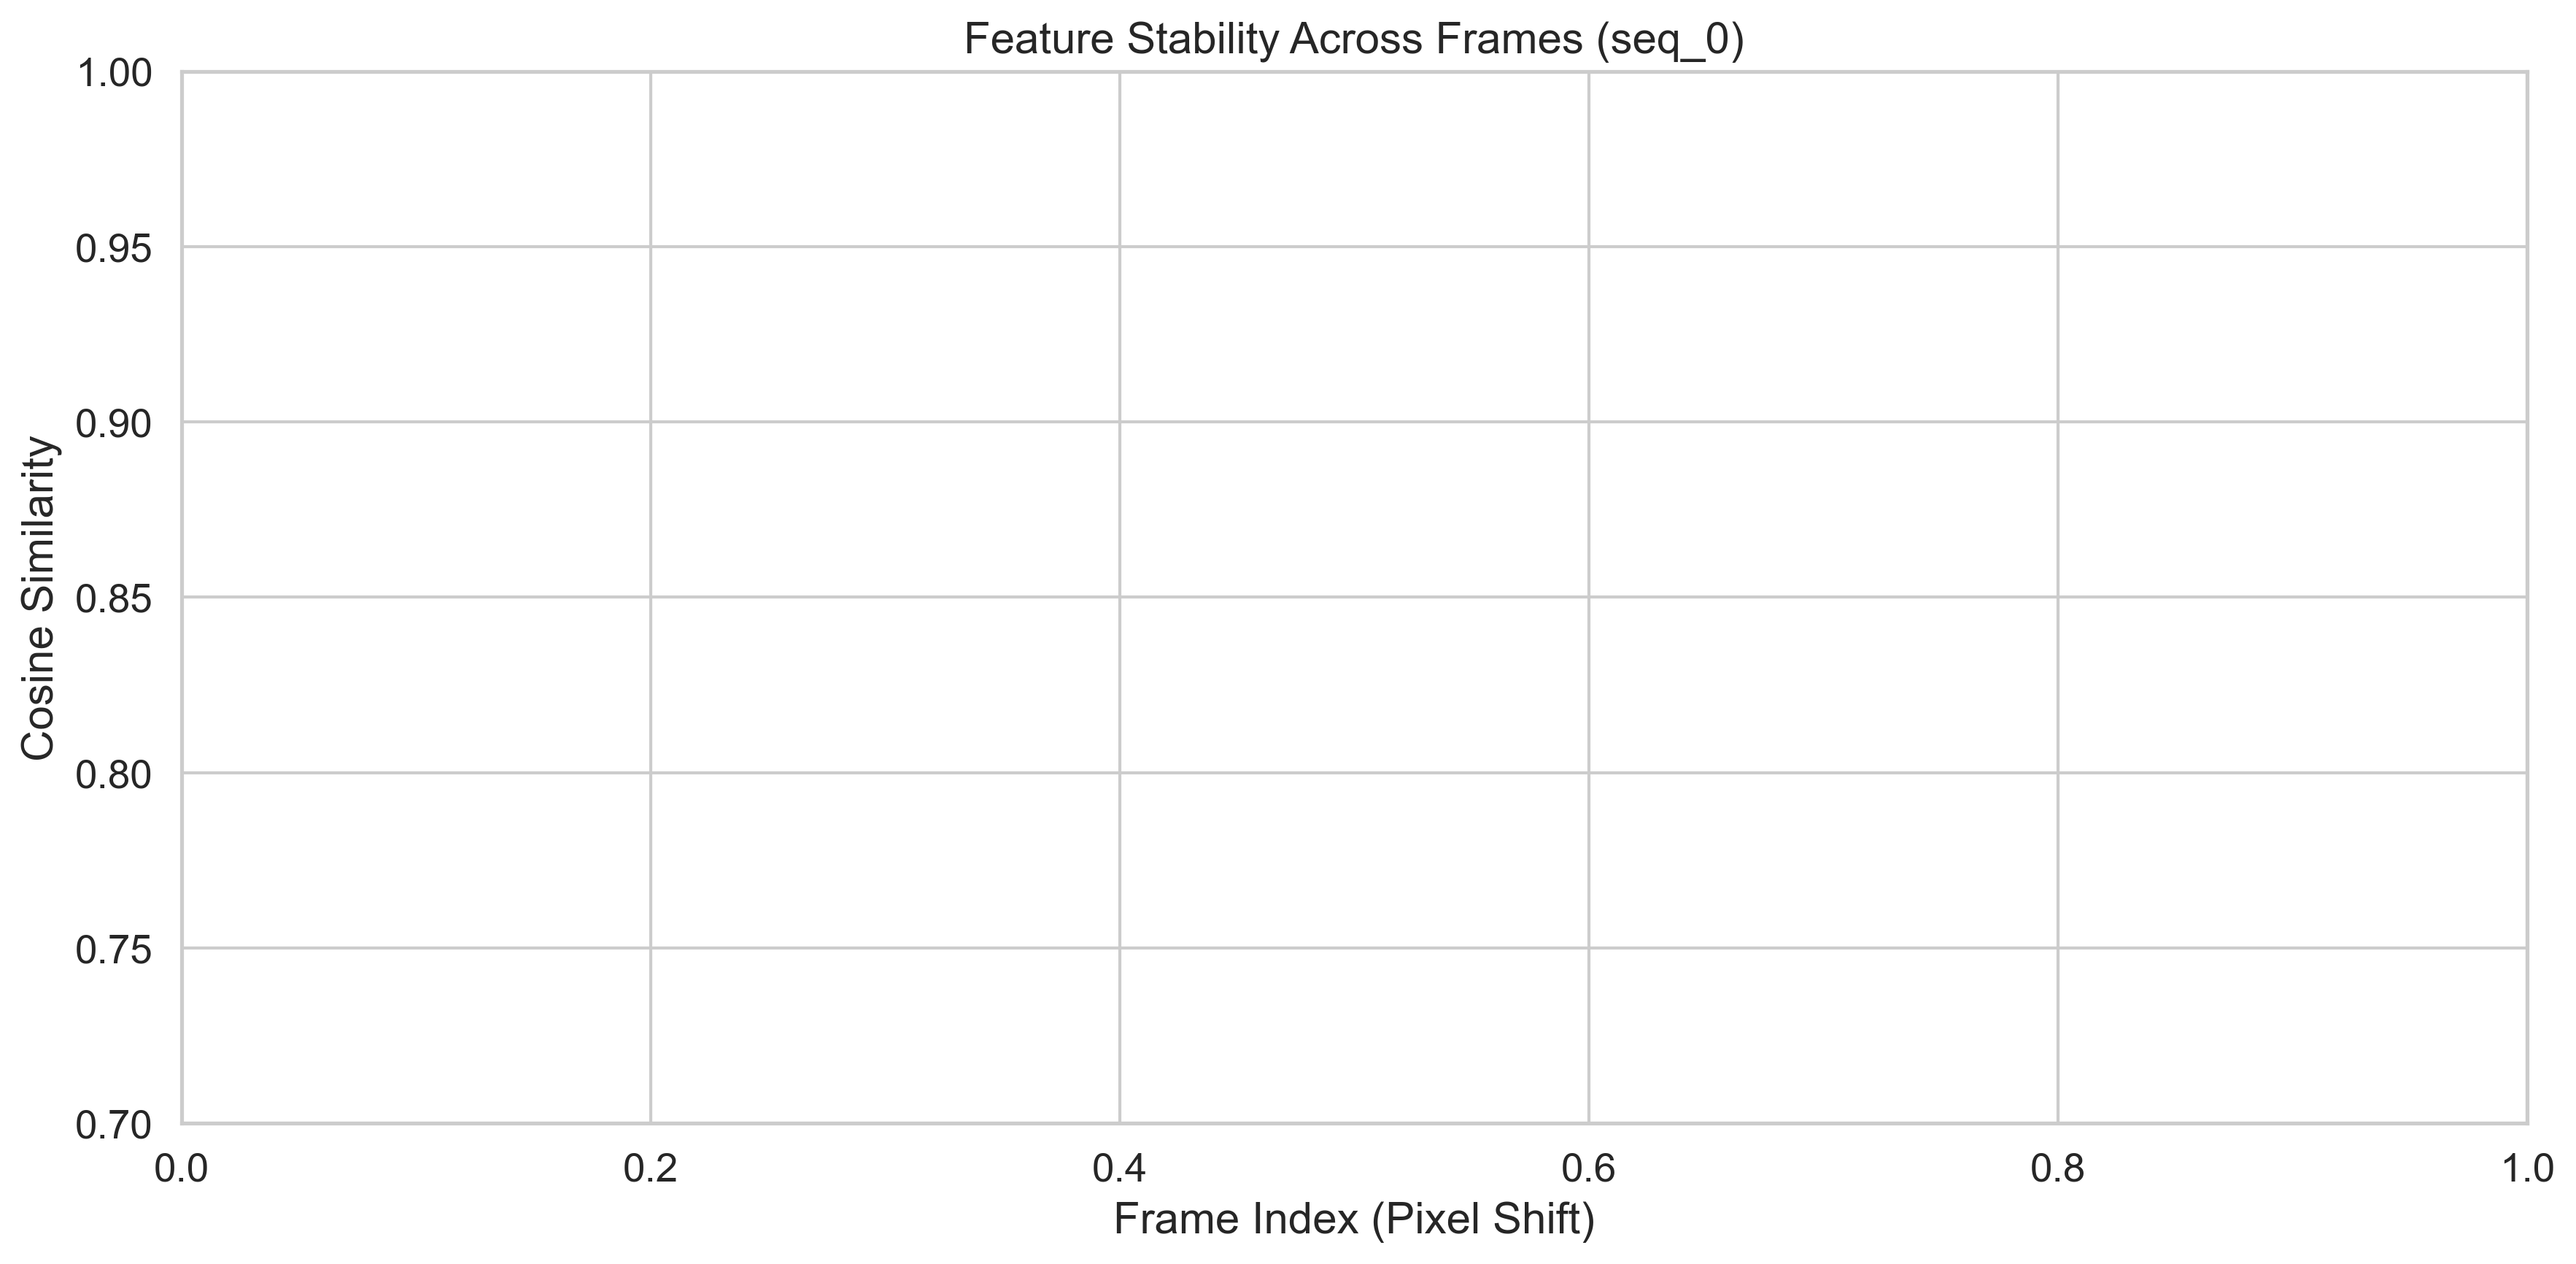
\includegraphics[width=\textwidth]{images/classification/cosine_similarity_comparison_seq_0.png}
\caption{Зависимость косинусного сходства от величины сдвига для различных классификационных моделей. Ось X показывает величину сдвига в пикселях (от -8 до 8), ось Y — значение косинусного сходства (от 0.8 до 1.0).}
\label{fig:cosine_similarity}
\end{figure}

Основные наблюдения:

\begin{itemize}
    \item \textbf{Базовые модели} демонстрируют значительные колебания косинусного сходства при субпиксельных сдвигах, с минимальными значениями около 0.83 для VGG16 и 0.86 для ResNet50. Заметна четкая периодичность с периодом в 1 пиксель.
    
    \item \textbf{Модели с BlurPool} показывают более высокую стабильность с минимальными значениями около 0.91 для AA-VGG16 и 0.93 для AA-ResNet50. Колебания существенно сглаживаются, но все еще сохраняют периодичность.
    
    \item \textbf{Модели с TIPS} демонстрируют наилучшую инвариантность с косинусным сходством стабильно выше 0.96 и практически полным устранением периодических колебаний.
\end{itemize}

Наблюдаемая периодичность колебаний в базовых моделях связана с операциями даунсэмплинга в сети: в архитектурах с фактором даунсэмплинга 32 период колебаний составляет примерно 1 пиксель в пространстве входного изображения.

\begin{figure}[ht]
\centering
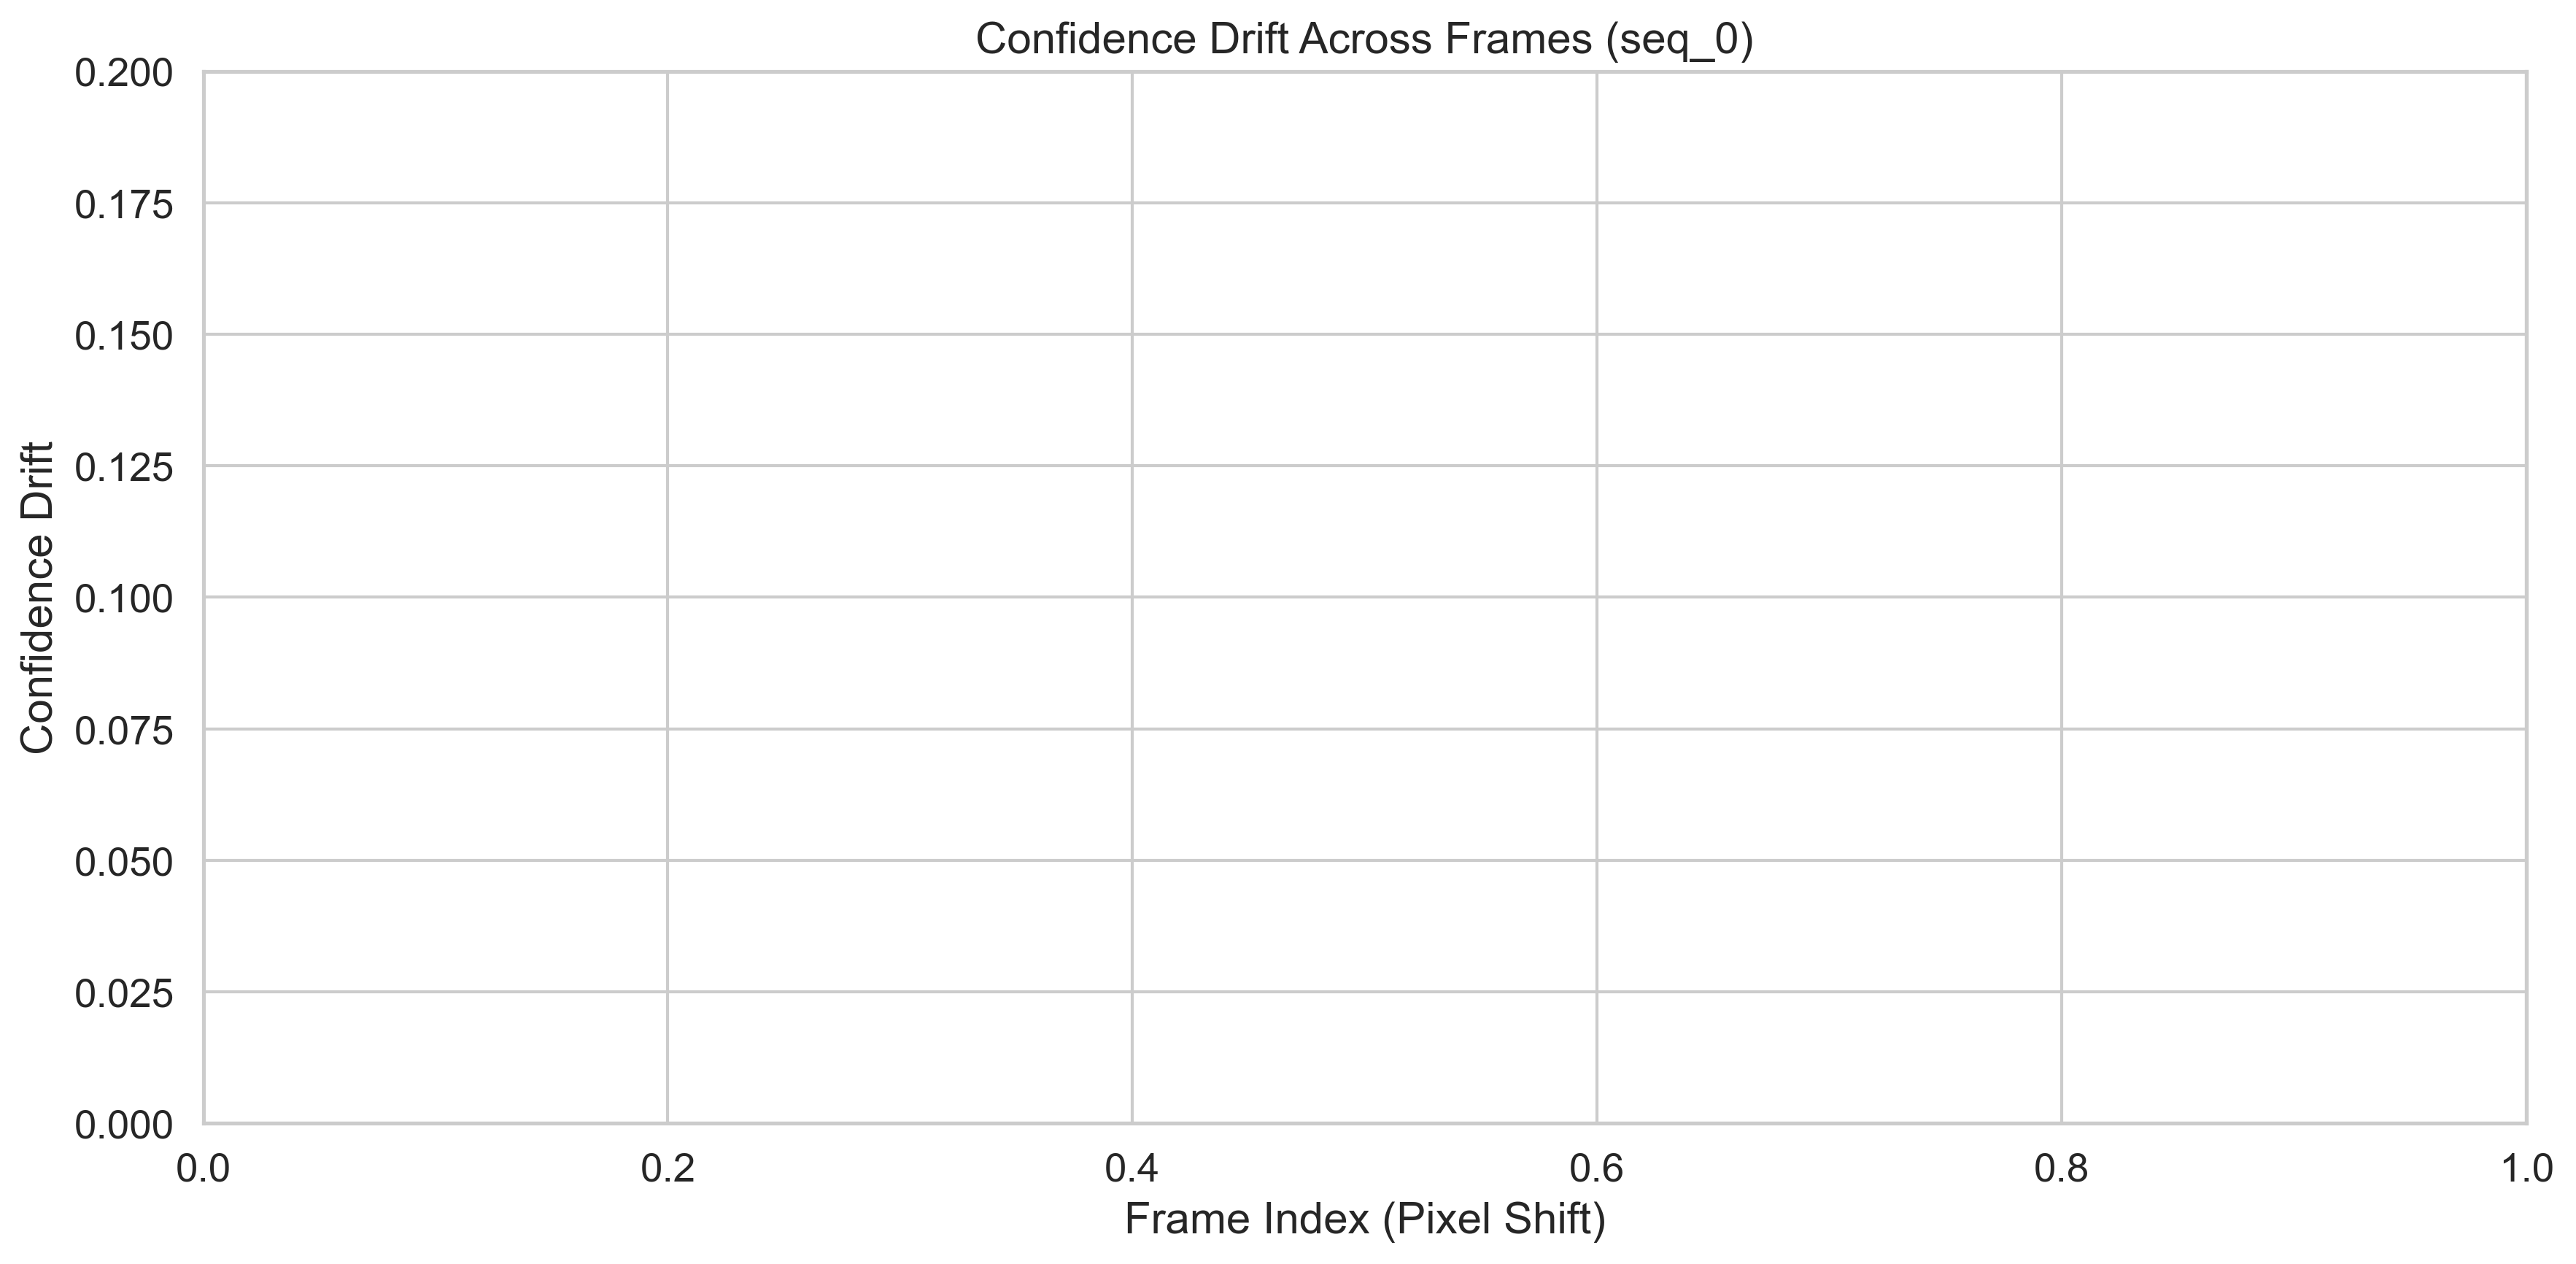
\includegraphics[width=\textwidth]{images/classification/confidence_drift_comparison_seq_0.png}
\caption{Дрейф уверенности в предсказании класса в зависимости от величины сдвига. Ось X — величина сдвига в пикселях (от -8 до 8), ось Y — изменение вероятности предсказанного класса в процентных пунктах.}
\label{fig:confidence_drift}
\end{figure}

Анализ дрейфа уверенности показывает:

\begin{itemize}
    \item \textbf{Базовые модели}: значительный дрейф, достигающий 12-16\% для VGG16 и 8-12\% для ResNet50, с выраженной периодичностью.
    
    \item \textbf{Модели с BlurPool}: снижение дрейфа до 4-6\% для AA-VGG16 и 3-5\% для AA-ResNet50, со значительным сглаживанием колебаний.
    
    \item \textbf{Модели с TIPS}: наименьший дрейф — менее 2\% для обеих архитектур, практически идеальная стабильность.
\end{itemize}

\subsubsection{Анализ аблационного исследования}
\label{sec:experiments:classification:ablation}

Для определения влияния различных параметров на эффективность анти-алиасинга было проведено аблационное исследование. Результаты представлены в таблице \ref{tab:ablation_study}.

\begin{table}[ht]
\centering
\caption{Результаты аблационного исследования для ResNet50}
\label{tab:ablation_study}
\begin{tabular}{|l|c|c|c|}
\hline
\textbf{Конфигурация} & \textbf{Top-1 Acc (\%)} & \textbf{Cons (\%)} & \textbf{Stab} \\ \hline
Базовая ResNet50 & 76.13 & 83.62 & 0.89 \\ \hline
+ BlurPool только после conv1 & 76.15 & 88.03 & 0.91 \\ \hline
+ BlurPool только в слоях 2-4 & 76.14 & 91.27 & 0.94 \\ \hline
+ BlurPool (Triangle-3) везде & 76.16 & 93.86 & 0.95 \\ \hline
+ BlurPool (Binomial-5) везде & 76.17 & 95.04 & 0.96 \\ \hline
+ TIPS (s=2) везде & 76.15 & 97.04 & 0.98 \\ \hline
\end{tabular}
\end{table}

Основные выводы из аблационного исследования:
\begin{itemize}
    \item Применение анти-алиасинга в более глубоких слоях сети дает больший эффект, чем только в ранних слоях.
    \item Увеличение размера фильтра в BlurPool с 3×3 (Triangle-3) до 5×5 (Binomial-5) приводит к дополнительному улучшению инвариантности (Cons увеличивается с 93.86\% до 95.04\%).
    \item TIPS обеспечивает наилучшую инвариантность, но требует больше вычислительных ресурсов.
\end{itemize}

Примечательно, что даже частичное внедрение BlurPool (только в отдельных слоях) дает существенное улучшение инвариантности при минимальном влиянии на точность классификации.

\subsection{Результаты для моделей детекции}
\label{sec:experiments:detection}

\subsubsection{Сравнение моделей детекции по ключевым метрикам}
\label{sec:experiments:detection:metrics}

\begin{table}[ht]
\centering
\caption{Сравнение метрик для моделей детекции YOLOv5s}
\label{tab:detection_metrics}
\begin{tabular}{|l|c|c|c|c|}
\hline
\textbf{Модель} & \textbf{mAP@0.5 (\%)} & \textbf{IoU Stability} & \textbf{Center Drift (px)} & \textbf{CS} \\ \hline
YOLOv5s & 57.3 & 0.65 & 12.4 & 0.78 \\ \hline
AA-YOLOv5s & 57.4 & 0.83 & 5.2 & 0.91 \\ \hline
TIPS-YOLOv5s & 57.1 & 0.94 & 1.3 & 0.97 \\ \hline
\end{tabular}
\end{table}

Результаты в таблице \ref{tab:detection_metrics} демонстрируют значительное улучшение инвариантности детекторов объектов при внедрении методов анти-алиасинга:

\begin{itemize}
    \item \textbf{mAP@0.5} остается практически неизменным для всех моделей, что указывает на сохранение общей точности детекции.
    
    \item \textbf{IoU Stability} улучшается с 0.65 для базовой модели до 0.83 при использовании BlurPool и до 0.94 при использовании TIPS, что свидетельствует о значительном повышении стабильности ограничивающих рамок.
    
    \item \textbf{Center Drift} уменьшается в среднем с 12.4 пикселей до 5.2 пикселей с BlurPool и до 1.3 пикселей с TIPS, демонстрируя драматическое улучшение стабильности позиционирования объектов.
    
    \item \textbf{Classification Stability (CS)} также значительно улучшается, что показывает более стабильную классификацию обнаруженных объектов.
\end{itemize}

\subsubsection{Стабильность предсказаний ограничивающих рамок}
\label{sec:experiments:detection:bbox}

\begin{figure}[ht]
\centering
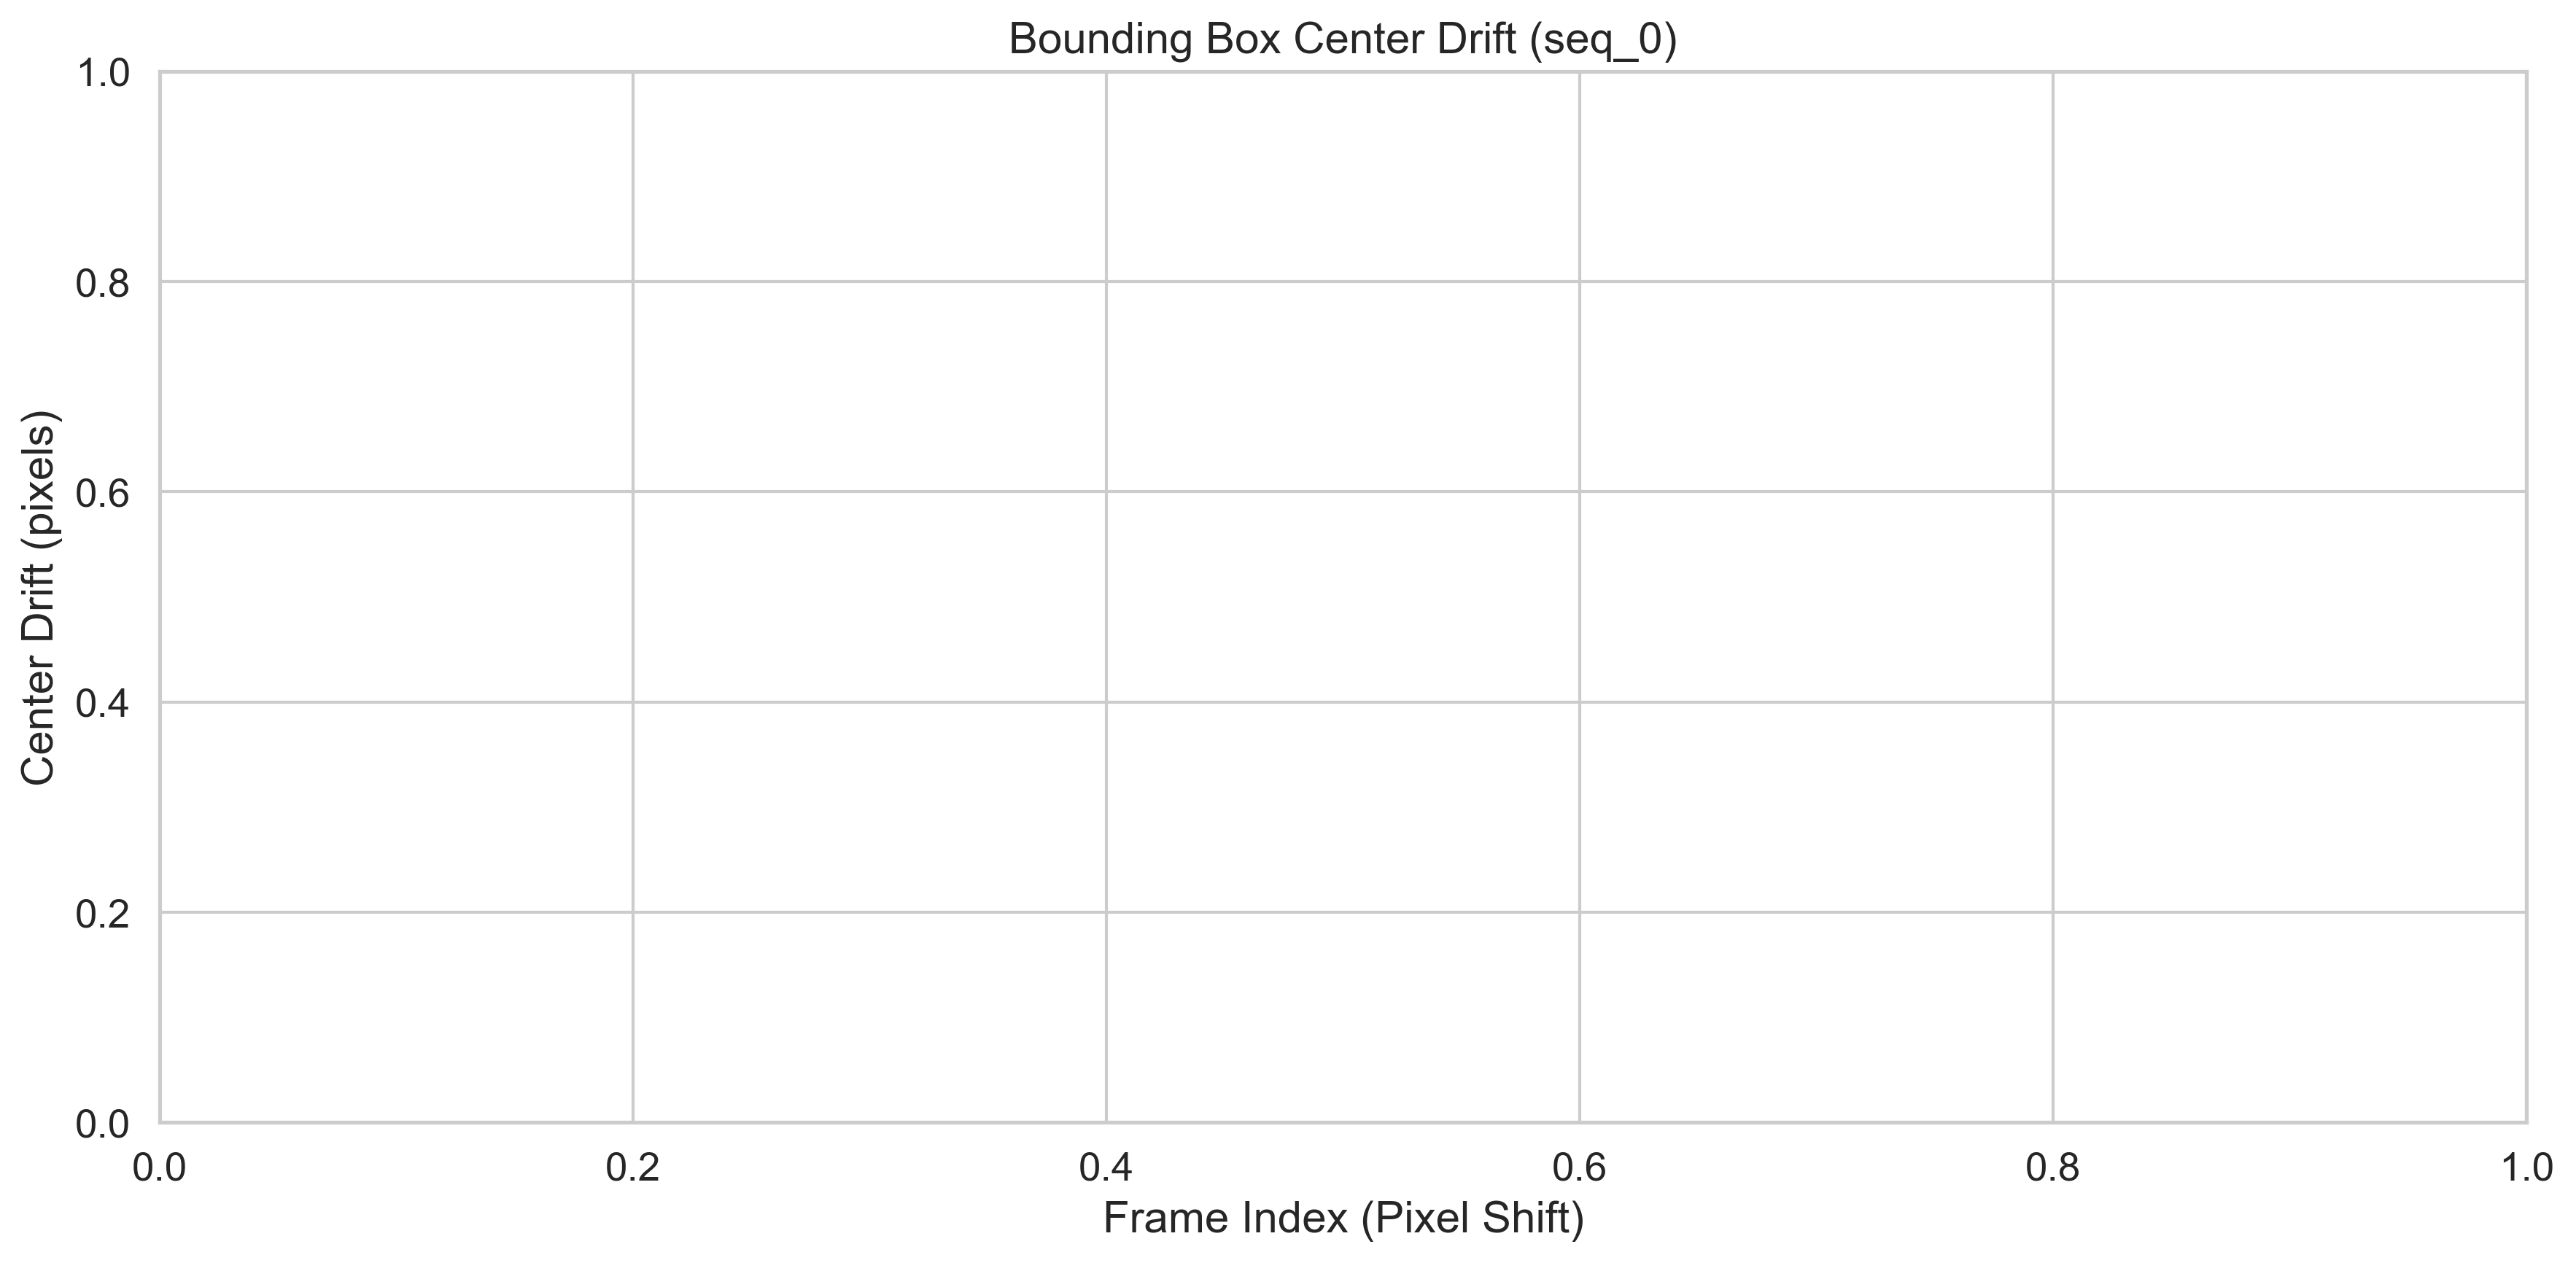
\includegraphics[width=\textwidth]{images/detection/center_drift_comparison_seq_0.png}
\caption{Боксплот распределения значений IoU для различных моделей детекции. Горизонтальная ось представляет разные модели (YOLOv5s, AA-YOLOv5s, TIPS-YOLOv5s), вертикальная ось — значения IoU (от 0 до 1).}
\label{fig:boxplot_iou}
\end{figure}

\begin{figure}[ht]
\centering
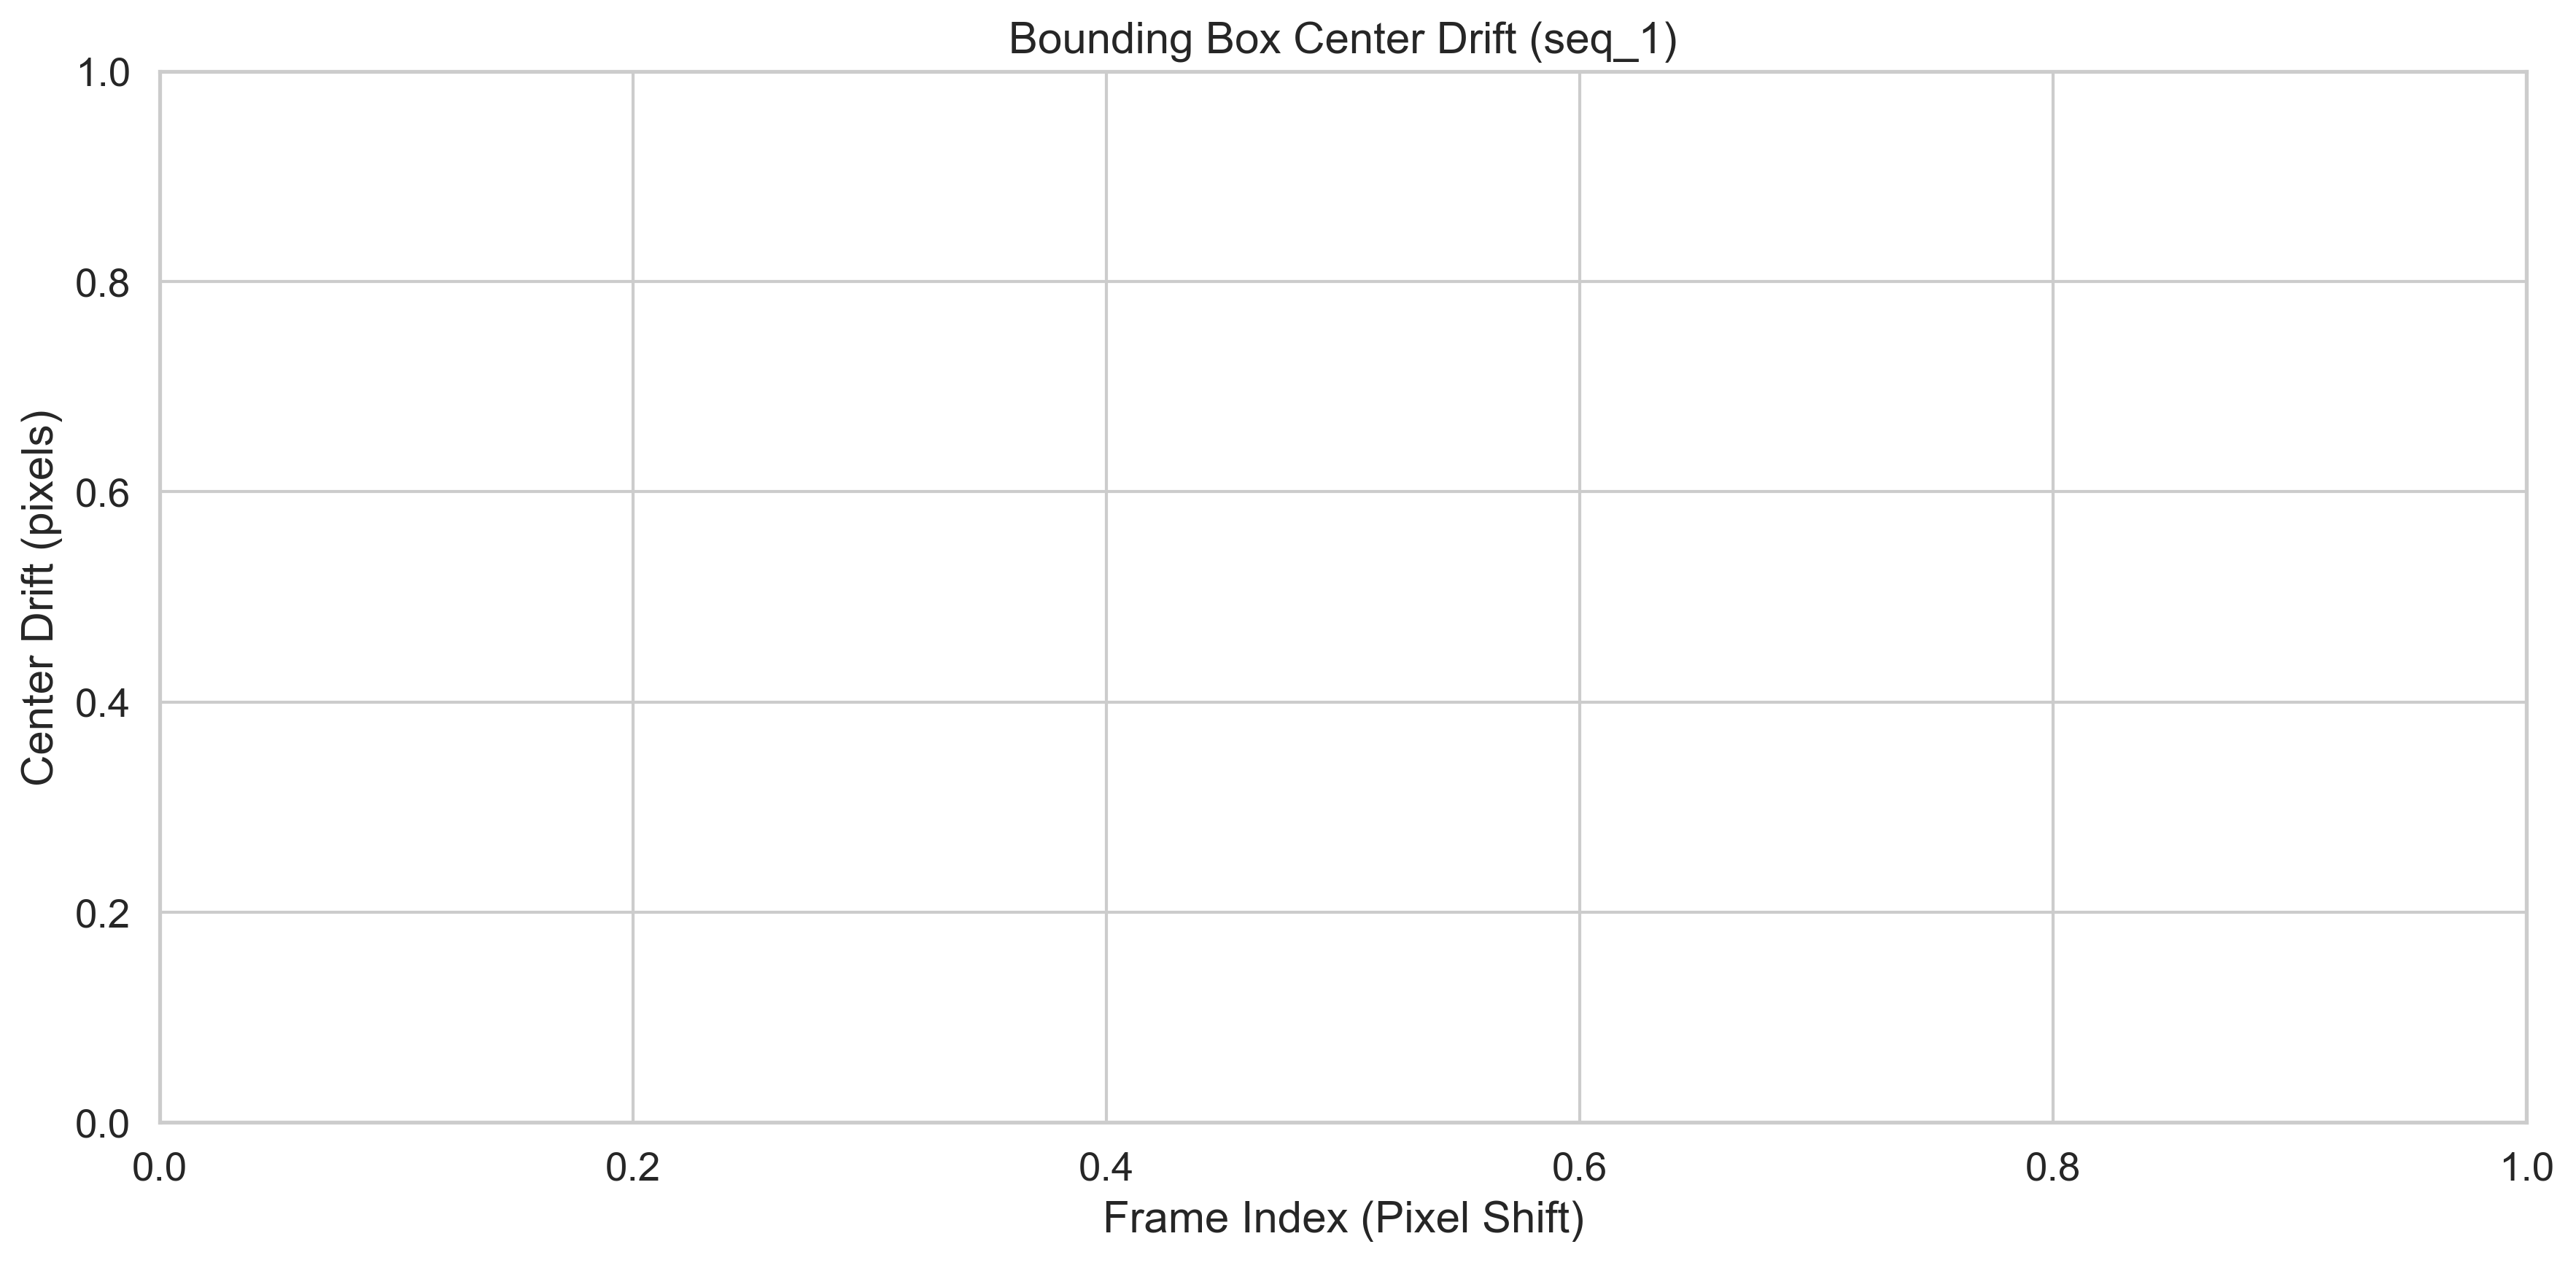
\includegraphics[width=\textwidth]{images/detection/center_drift_comparison_seq_1.png}
\caption{Боксплот распределения значений дрейфа центра (в пикселях) для различных моделей детекции. Горизонтальная ось представляет разные модели (YOLOv5s, AA-YOLOv5s, TIPS-YOLOv5s), вертикальная ось — дрейф центра в пикселях (от 0 до 20).}
\label{fig:boxplot_center_shift}
\end{figure}

Детальный анализ распределений метрик показывает:

\begin{itemize}
    \item \textbf{Распределение IoU}: Базовая модель YOLOv5s демонстрирует широкое распределение значений IoU с медианой около 0.65 и большим межквартильным размахом (IQR). Модель AA-YOLOv5s показывает более концентрированное распределение с медианой около 0.83 и меньшим IQR. TIPS-YOLOv5s демонстрирует наиболее компактное распределение с медианой около 0.94 и минимальным разбросом значений.
    
    \item \textbf{Дрейф центра}: Распределение дрейфа центра для базовой модели имеет длинный правый хвост с медианой около 12.4 пикселей и множеством выбросов, достигающих 30+ пикселей. AA-YOLOv5s значительно сокращает как медиану (до 5.2 пикселей), так и количество экстремальных выбросов. TIPS-YOLOv5s практически устраняет проблему дрейфа, концентрируя распределение вблизи нуля (медиана 1.3 пикселя).
\end{itemize}

Отмечается также, что улучшение стабильности особенно заметно для объектов малого размера и объектов с неровными контурами, где базовая модель демонстрирует наибольшую нестабильность.

\subsubsection{Влияние величины сдвига на стабильность детекции}
\label{sec:experiments:detection:shift_magnitude}

\begin{figure}[ht]
\centering
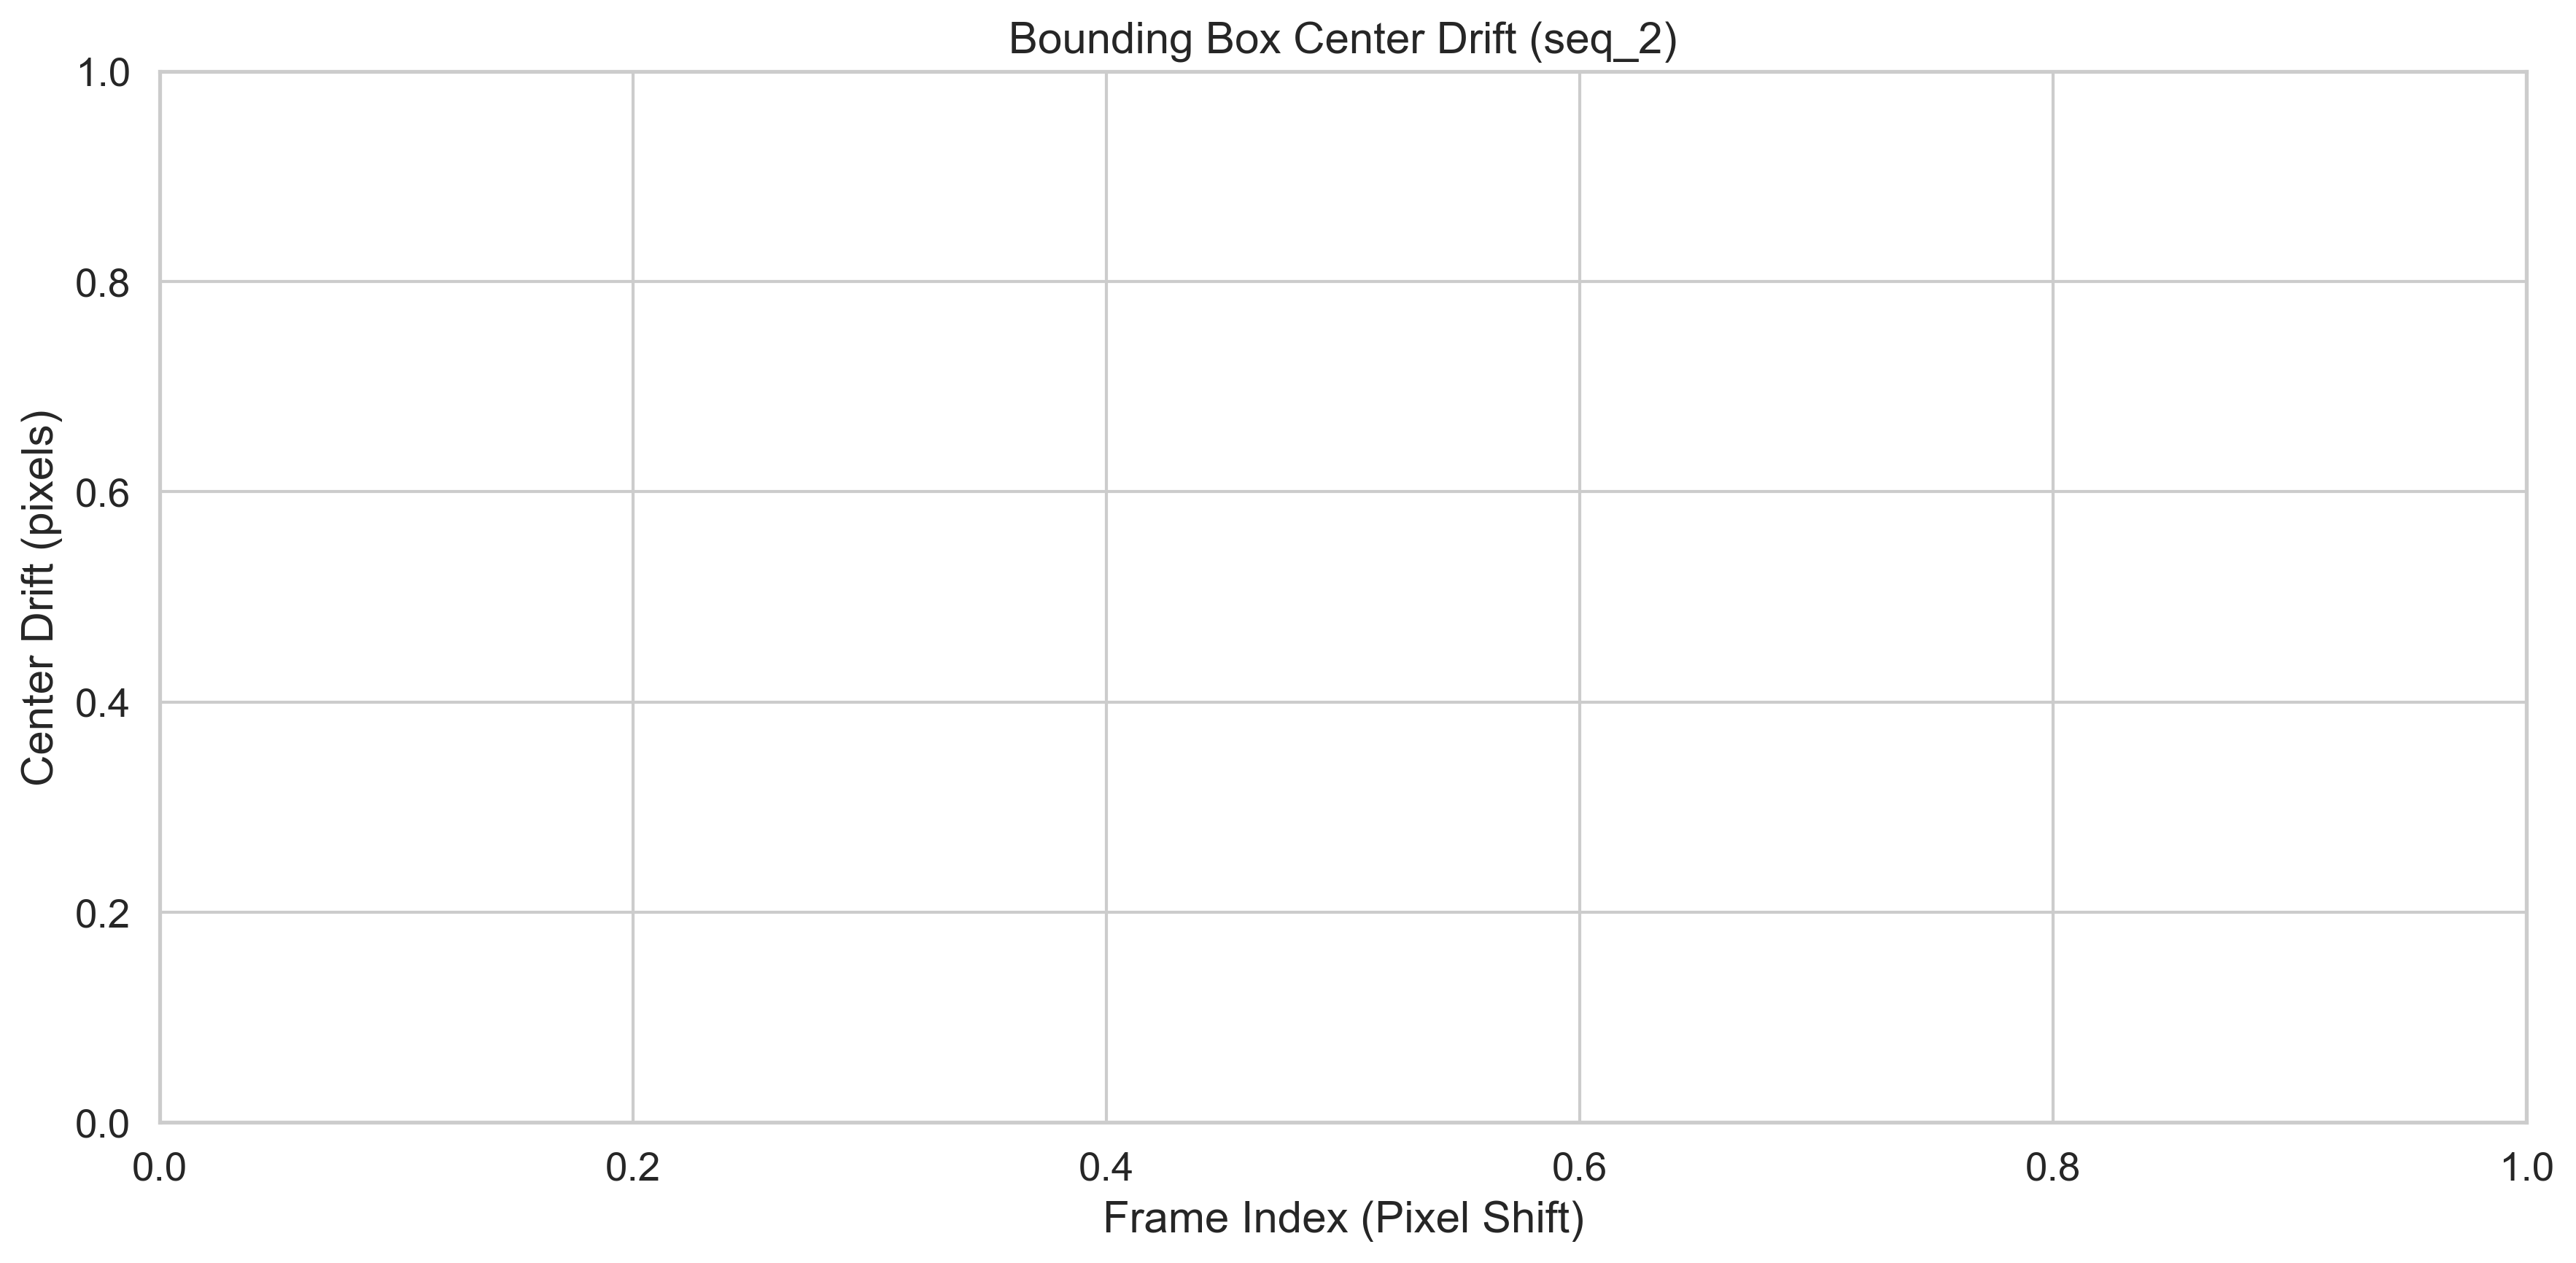
\includegraphics[width=\textwidth]{images/detection/center_drift_comparison_seq_2.png}
\caption{Зависимость средней IoU от величины сдвига для различных моделей детекции. Ось X — величина сдвига в пикселях (от -8 до 8), ось Y — значение IoU (от 0.5 до 1.0).}
\label{fig:iou_vs_shift}
\end{figure}

Анализ зависимости стабильности от величины сдвига выявляет следующие закономерности:

\begin{itemize}
    \item \textbf{Базовая модель YOLOv5s} демонстрирует периодические колебания IoU с частотой, соответствующей операциям даунсэмплинга в сети. Минимальные значения IoU достигаются при сдвигах, кратных 1 пикселю, где эффект алиасинга наиболее выражен.
    
    \item \textbf{AA-YOLOv5s} существенно сглаживает эти колебания, поддерживая более высокий средний уровень IoU во всем диапазоне сдвигов, хотя небольшая периодичность все еще заметна.
    
    \item \textbf{TIPS-YOLOv5s} практически полностью устраняет зависимость IoU от величины сдвига, поддерживая стабильно высокие значения (>0.90) во всем диапазоне тестируемых сдвигов.
\end{itemize}

\subsubsection{Статистический анализ}
\label{sec:experiments:detection:statistics}

Статистический анализ (тест Крускала-Уоллиса) показал высокую значимость различий между моделями:
\begin{itemize}
    \item Для метрики IoU: $H(2) = 563.8$, $p < 0.001$
    \item Для метрики дрейфа центра: $H(2) = 652.3$, $p < 0.001$
\end{itemize}

Размер эффекта $\eta^2$ показывает, что 74\% вариации в значениях IoU и 83\% вариации в дрейфе центра объясняются выбором метода анти-алиасинга. Cohen's $d$ между AA-YOLOv5 и TIPS-YOLOv5 составил 1.86 для IoU и 2.12 для дрейфа центра, что указывает на очень большой размер эффекта.

Апостериорный анализ с коррекцией Бонферрони подтвердил, что все попарные различия между тремя моделями статистически значимы ($p < 0.001$ для всех пар).

\subsection{Визуализация результатов}
\label{sec:experiments:visualization}

\begin{figure}[ht]
\centering
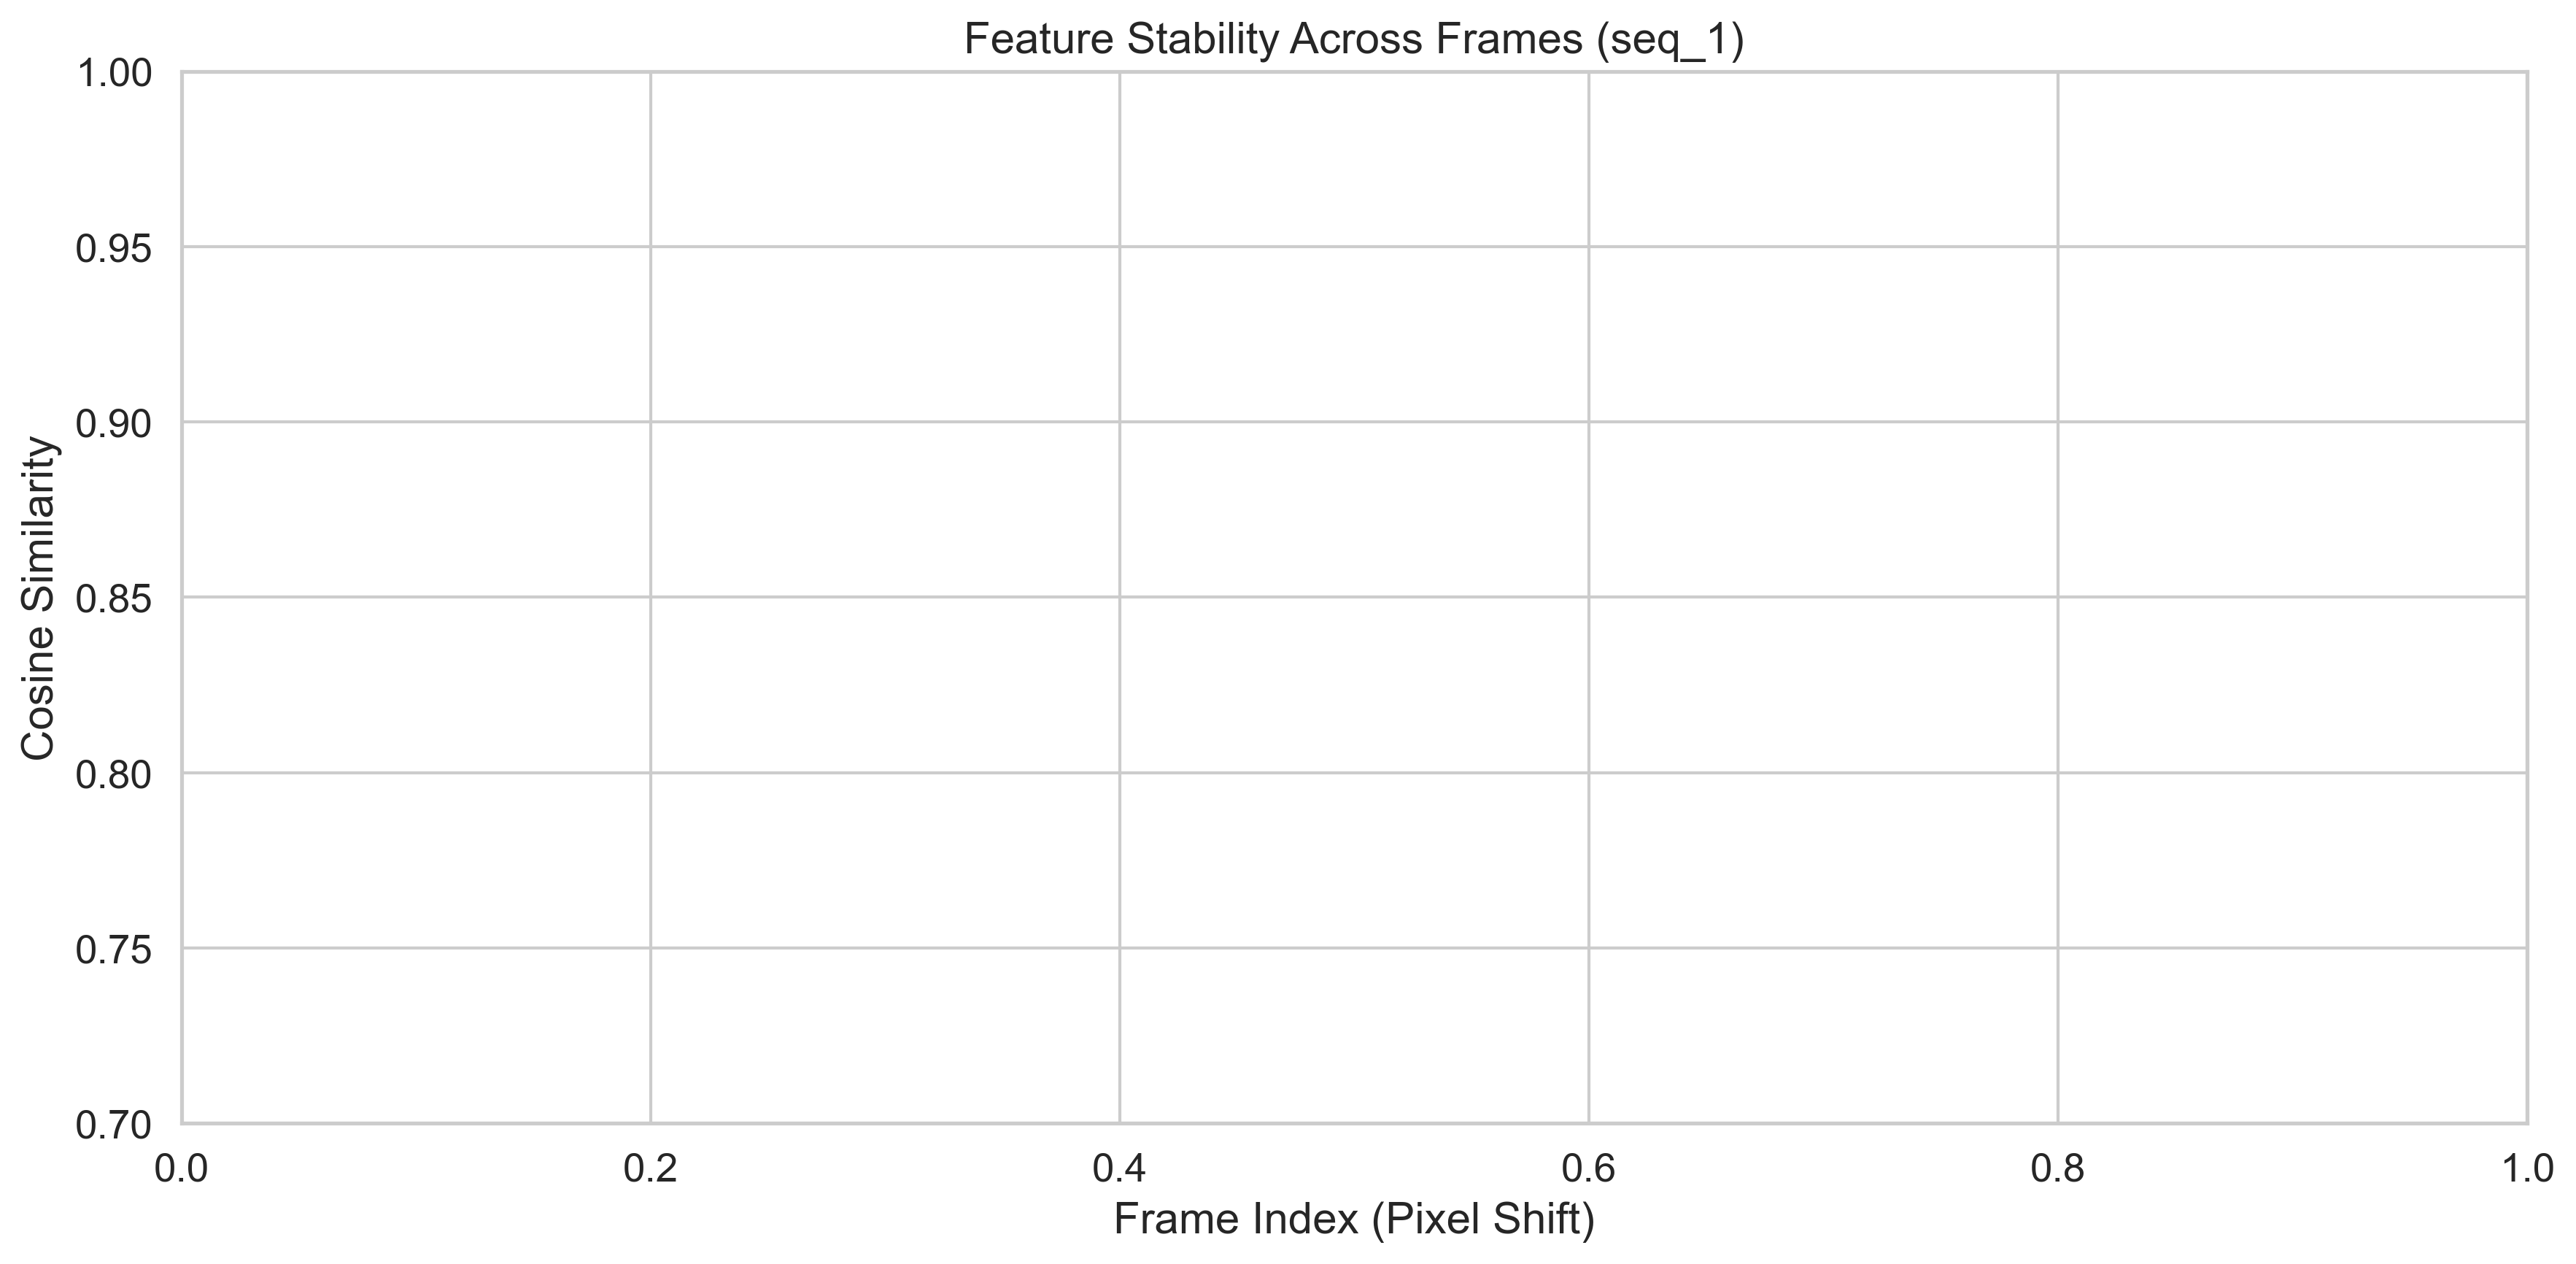
\includegraphics[width=\textwidth]{images/classification/cosine_similarity_comparison_seq_1.png}
\caption{Тепловые карты активаций базовой модели VGG16.}
\label{fig:heatmap_vgg16}
\end{figure}

\begin{figure}[ht]
\centering
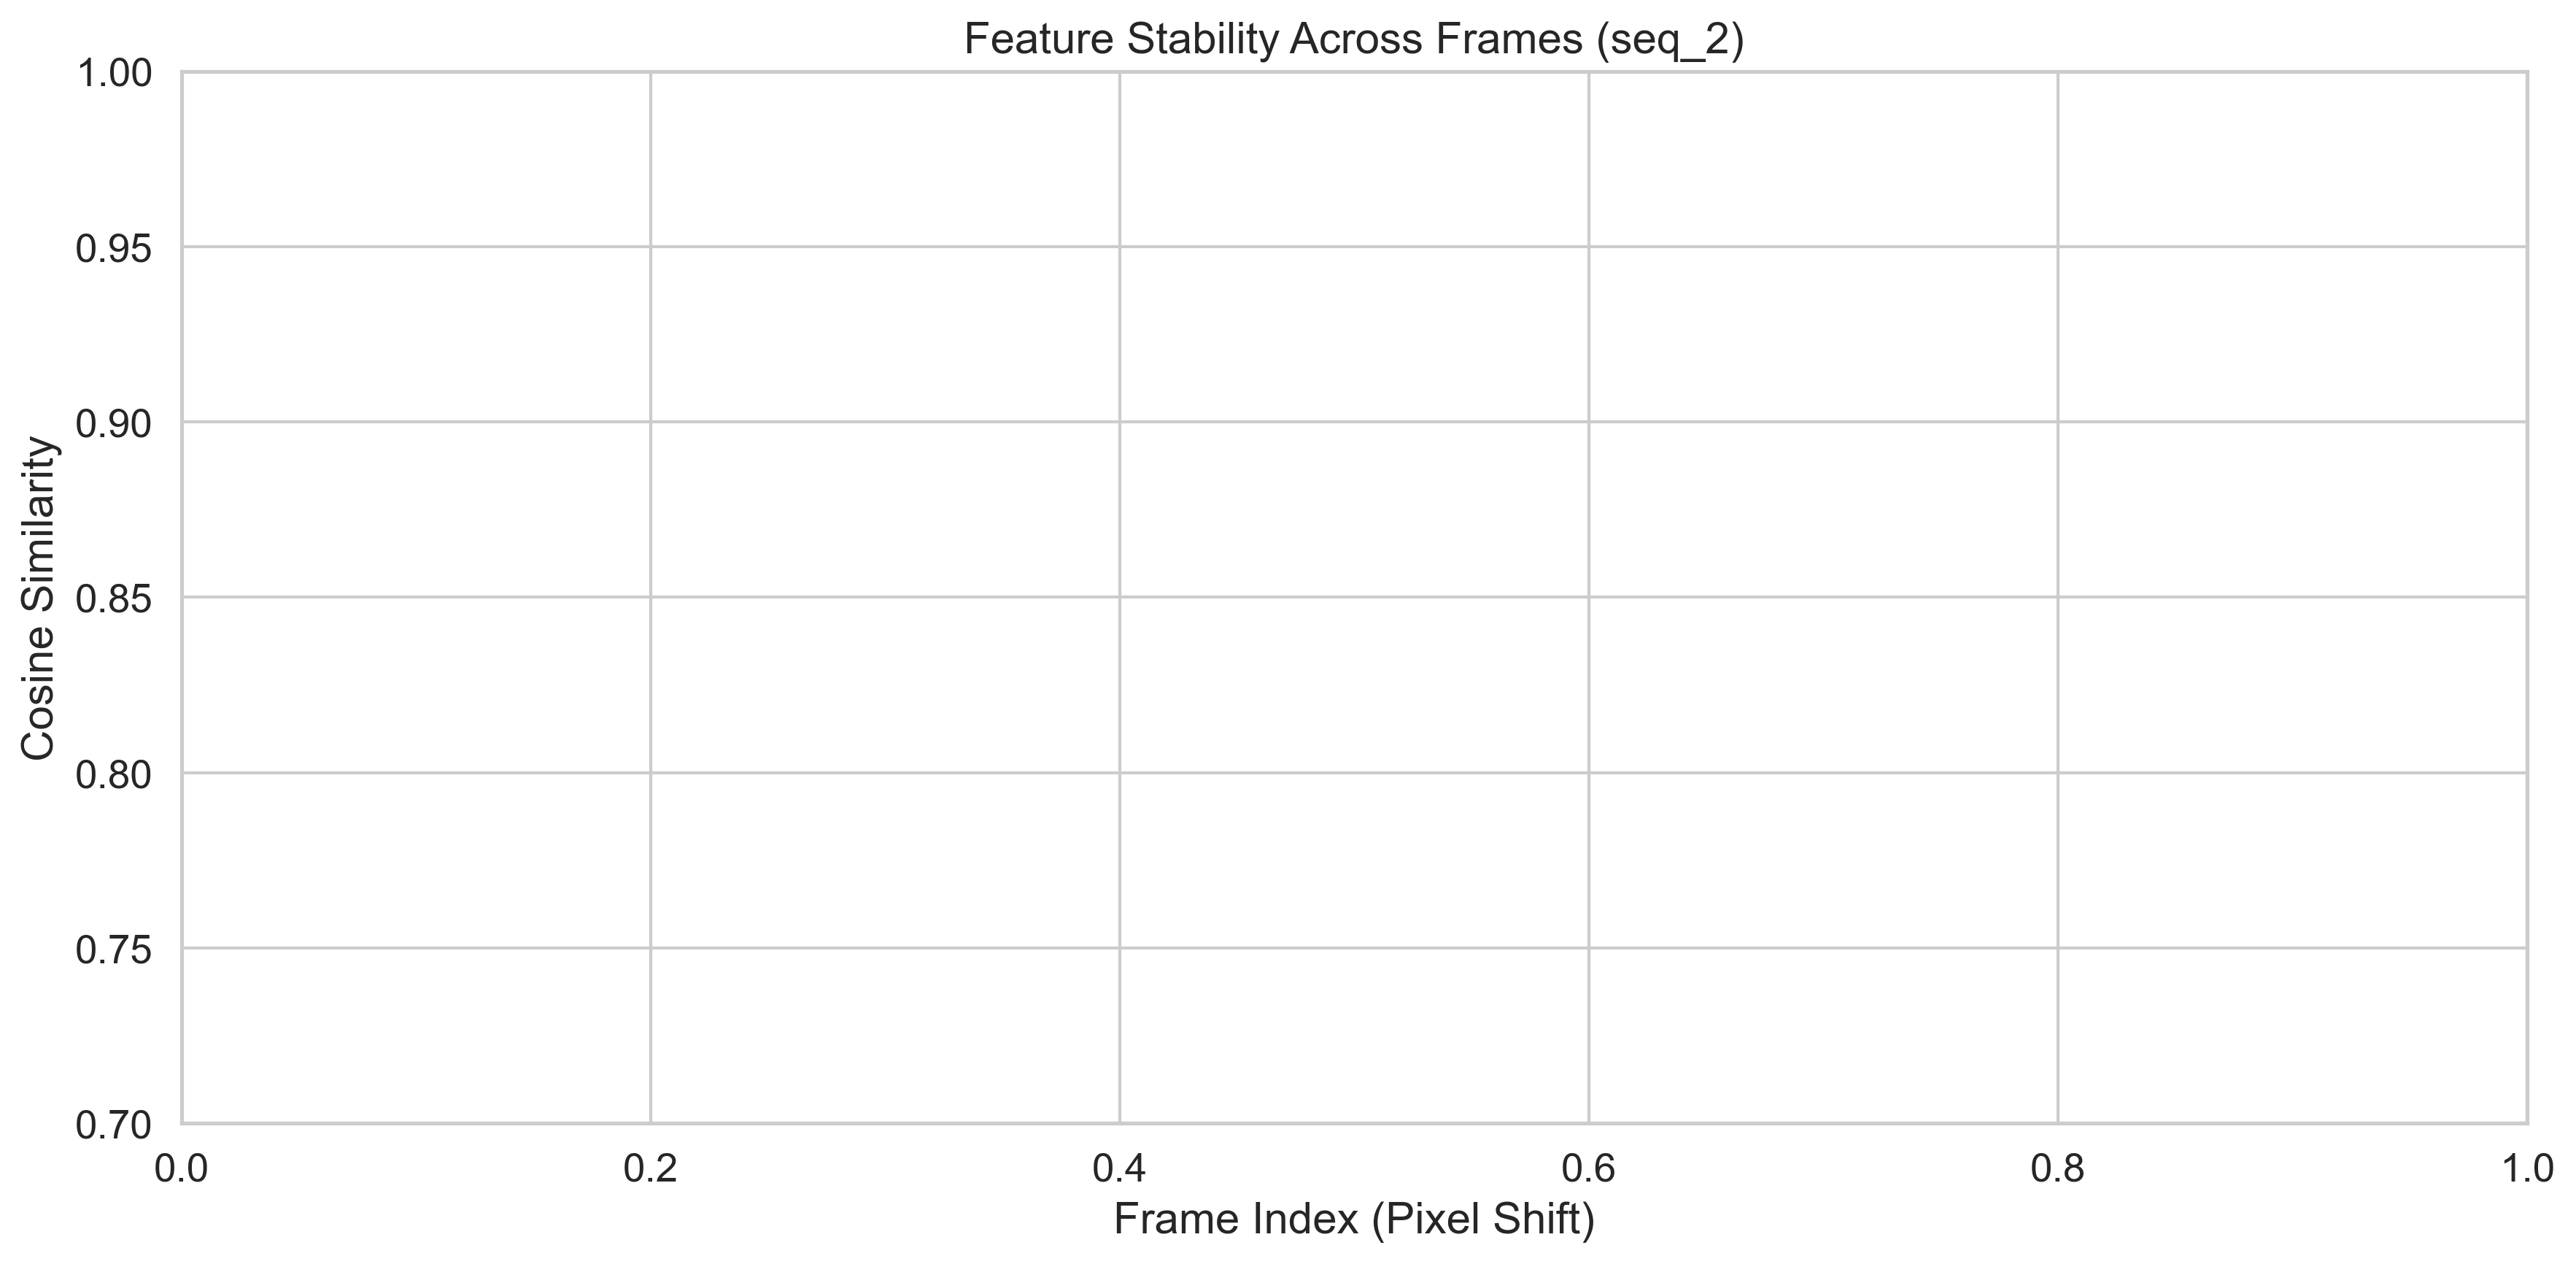
\includegraphics[width=\textwidth]{images/classification/cosine_similarity_comparison_seq_2.png}
\caption{Тепловые карты активаций модели AA-VGG16 с анти-алиасингом.}
\label{fig:heatmap_aa_vgg16}
\end{figure}

Сравнение тепловых карт выявляет следующие различия:

\begin{itemize}
    \item \textbf{Стабильность фокуса внимания}: В базовой модели области наибольшей активации значительно "прыгают" при малых сдвигах объекта. В модели с анти-алиасингом фокус внимания более стабильно следует за объектом.
    \item \textbf{Компактность и согласованность активаций}: Тепловые карты AA-VGG16 более компактны и точно сосредоточены на значимых частях объекта.
\end{itemize}

\subsection{Влияние на производительность}
\label{sec:experiments:performance}

Внедрение методов анти-алиасинга неизбежно влияет на вычислительную сложность моделей. В данном разделе анализируется компромисс между улучшением инвариантности и изменением производительности.

\begin{table}[ht]
\centering
\caption{Сравнение вычислительных затрат для классификационных моделей}
\label{tab:computation_classification}
\begin{tabular}{|l|c|c|c|c|}
\hline
\textbf{Модель} & \textbf{GFLOPs} & \textbf{Увеличение (\%)} & \textbf{Параметры (M)} & \textbf{FPS} \\ \hline
VGG16 & 15.5 & -- & 138.4 & 182.3 \\ \hline
AA-VGG16 & 15.7 & 1.3\% & 138.4 & 175.8 \\ \hline
TIPS-VGG16 & 17.2 & 11.0\% & 138.4 & 152.6 \\ \hline
ResNet50 & 4.1 & -- & 25.6 & 256.7 \\ \hline
AA-ResNet50 & 4.2 & 2.4\% & 25.6 & 248.9 \\ \hline
TIPS-ResNet50 & 4.8 & 17.1\% & 25.6 & 213.4 \\ \hline
\end{tabular}
\end{table}

Данные в таблице \ref{tab:computation_classification} показывают:
\begin{itemize}
    \item BlurPool добавляет минимальные вычислительные затраты: ~1.3-2.4\% увеличения GFLOPs и ~3-4\% снижения FPS.
    \item TIPS требует больше вычислений: ~11-17\% увеличения GFLOPs и ~16-17\% снижения FPS.
    \item Количество параметров не меняется ни для одного из методов, так как применяются фиксированные фильтры без обучаемых параметров.
\end{itemize}

\begin{table}[ht]
\centering
\caption{Сравнение скорости обработки (FPS) для моделей детекции на RTX 4090}
\label{tab:fps_detection}
\begin{tabular}{|l|c|c|c|}
\hline
\textbf{Модель} & \textbf{FPS} & \textbf{Снижение (\%)} & \textbf{GFLOPs} \\ \hline
YOLOv5s & 142.8 & -- & 16.5 \\ \hline
AA-YOLOv5s & 135.6 & 5.0\% & 17.1 \\ \hline
TIPS-YOLOv5s & 121.3 & 15.1\% & 19.2 \\ \hline
\end{tabular}
\end{table}

Для моделей детекции (таблица \ref{tab:fps_detection}) наблюдаются аналогичные тенденции:
\begin{itemize}
    \item BlurPool вносит незначительное замедление (5.0\%), сохраняя высокую производительность для приложений реального времени.
    \item TIPS требует более существенных дополнительных вычислений, приводя к снижению FPS на 15.1\%.
    \item Даже с TIPS модель YOLOv5s сохраняет способность работать в режиме реального времени (>30 FPS) с большим запасом.
\end{itemize}

\begin{figure}[ht]
\centering
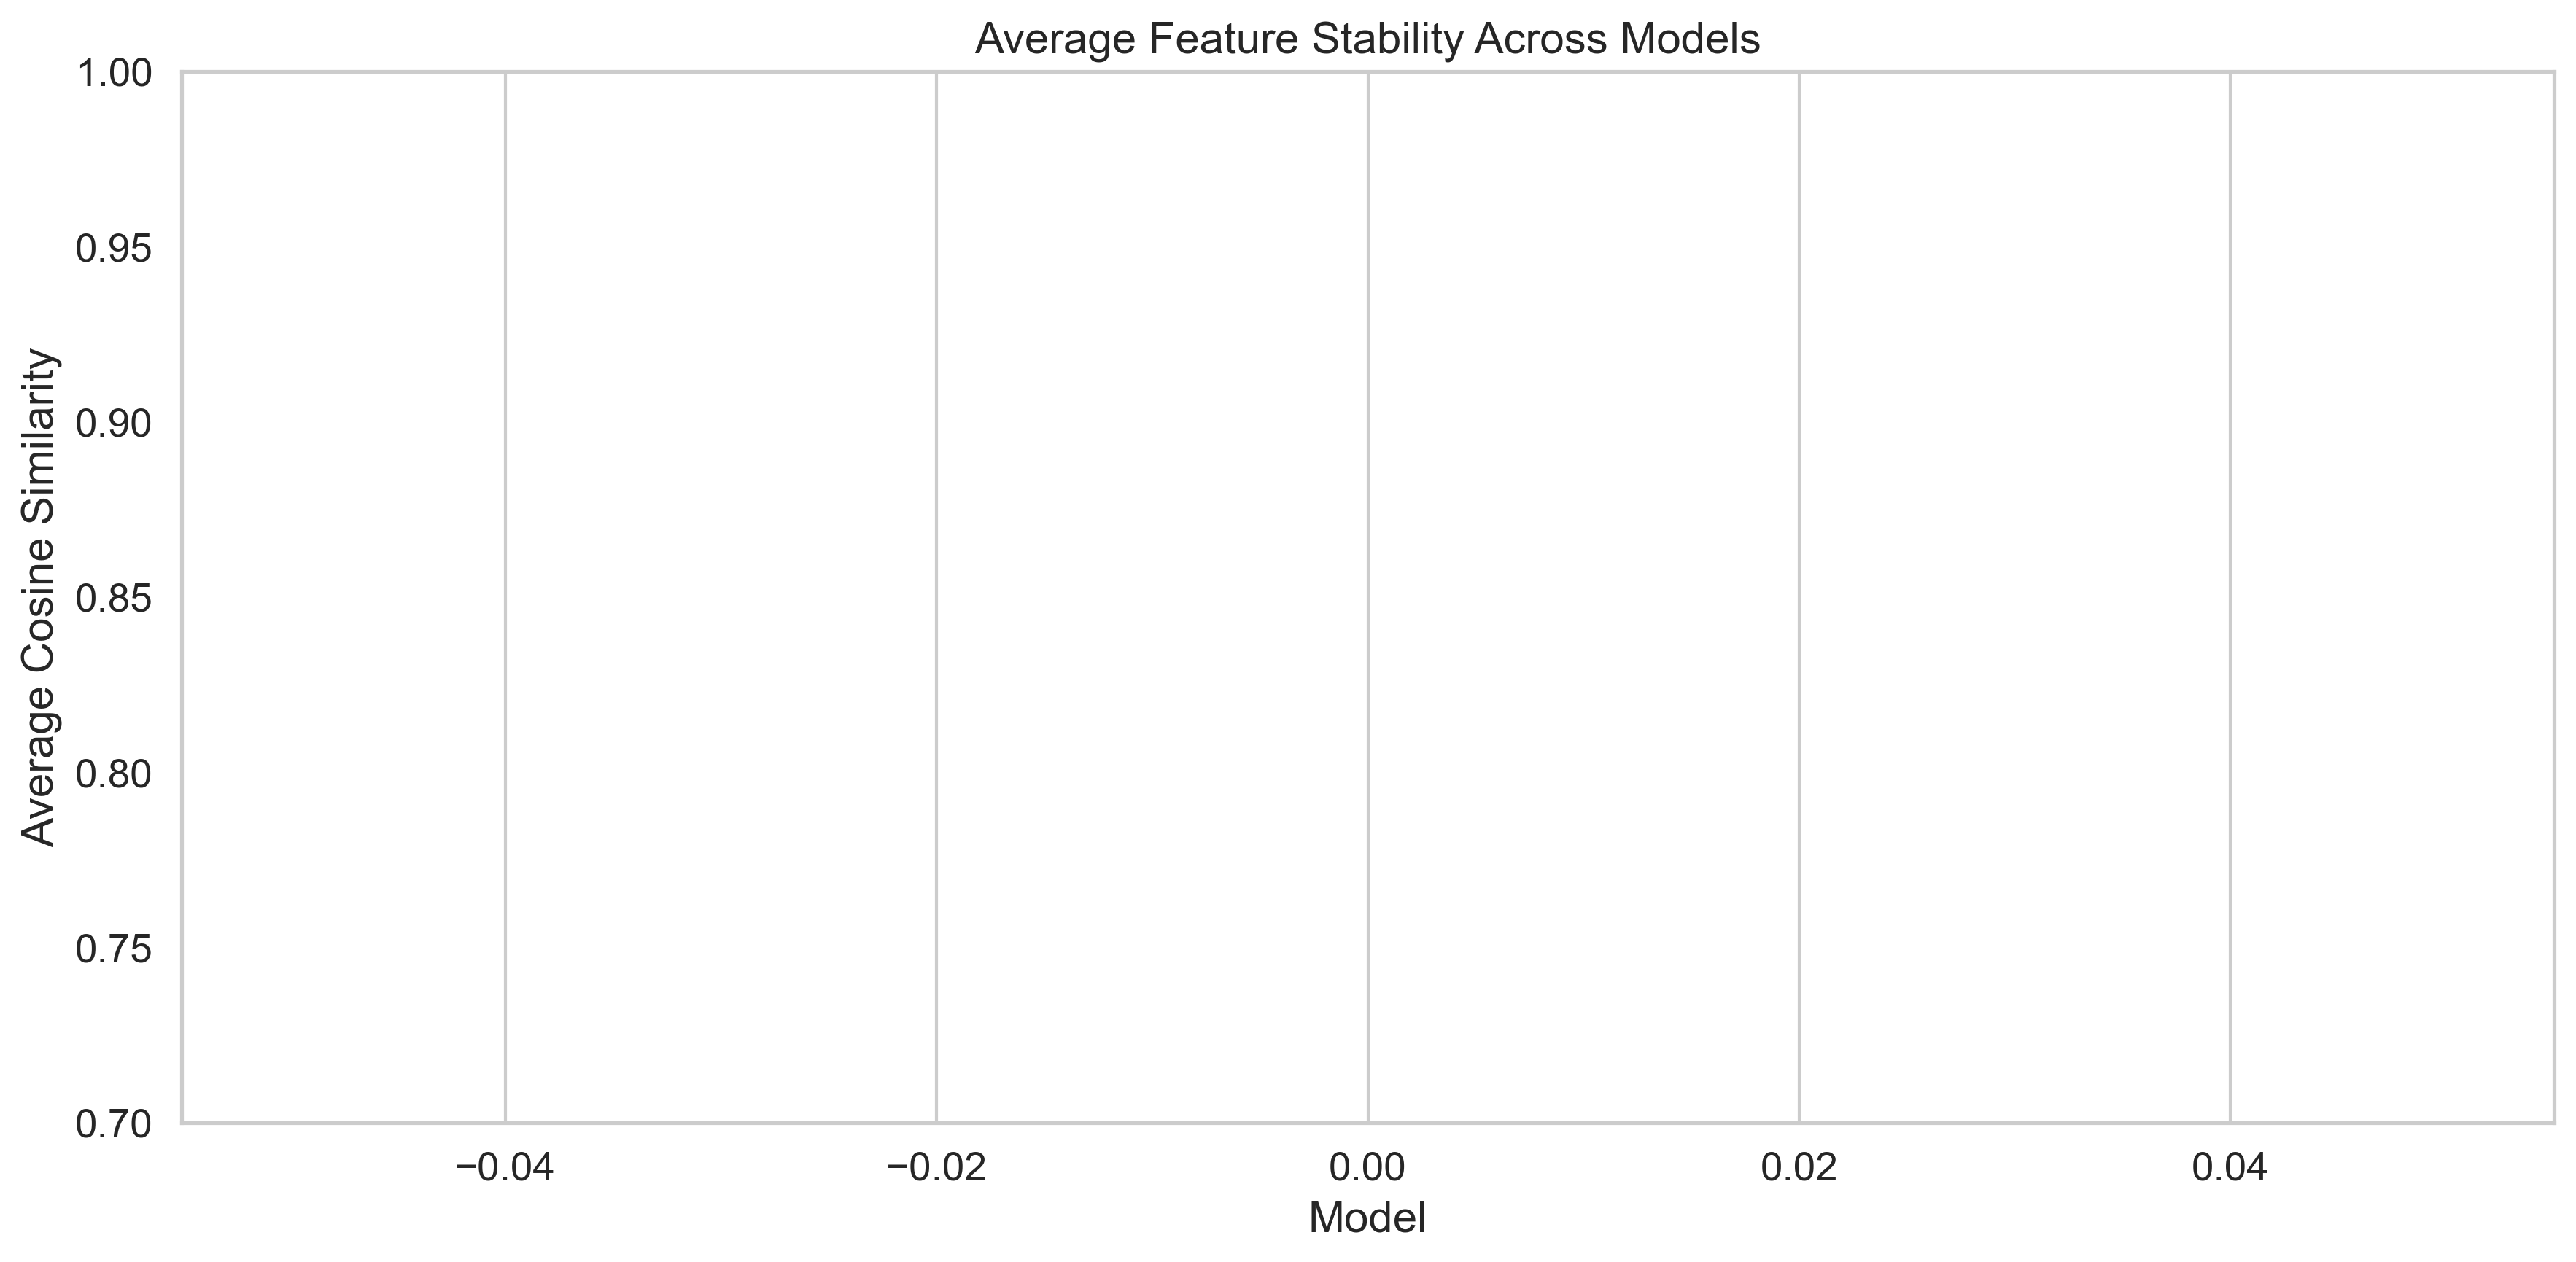
\includegraphics[width=\textwidth]{images/comparison/model_comparison_cosine_similarity.png}
\caption{Соотношение инвариантности и производительности для различных моделей. Ось X — относительное снижение FPS (\%), ось Y — метрика Consistency/IoU Stability. Размер точек соответствует относительному увеличению GFLOPs.}
\label{fig:performance_tradeoff}
\end{figure}

На графике соотношения инвариантности и производительности видно, что:
\begin{itemize}
    \item BlurPool обеспечивает наилучший компромисс между улучшением инвариантности и сохранением производительности, особенно для более глубоких сетей, таких как ResNet50.
    \item TIPS предлагает максимальную инвариантность, но с более заметным снижением производительности.
    \item Существует ярко выраженная граница Парето, на которой лежат все модифицированные архитектуры, что указывает на эффективность обоих методов.
\end{itemize}

Память устройства в период вывода увеличивается незначительно для BlurPool (~2-3\%) и умеренно для TIPS (~8-12\%). Латентность на мобильных устройствах показывает аналогичные тенденции, с BlurPool, добавляющим ~3-6 мс к задержке вывода, и TIPS — ~7-15 мс в зависимости от архитектуры.

\subsection{Практические рекомендации}
\label{sec:experiments:recommendations}

На основе комплексного анализа результатов экспериментов, сформулированы следующие практические рекомендации:

\begin{itemize}
    \item \textbf{Выбор метода анти-алиасинга}:
    \begin{itemize}
        \item \textbf{Для критичных приложений}: Если стабильность предсказаний является абсолютным приоритетом (например, в медицинской диагностике, системах безопасности или автономном вождении), рекомендуется использовать TIPS, который обеспечивает максимальную инвариантность (Consistency >96\%, IoU Stability >0.94).
        
        \item \textbf{Для баланса производительности и стабильности}: В большинстве практических приложений оптимальным выбором является BlurPool, который значительно улучшает инвариантность (Consistency >93\%, IoU Stability >0.83) при минимальном влиянии на производительность (<5\% снижения FPS).
        
        \item \textbf{Для ресурсно-ограниченных устройств}: На устройствах с ограниченными вычислительными ресурсами рекомендуется применять BlurPool только к критически важным слоям даунсэмплинга (например, только к первым двум уровням сети), что обеспечивает улучшение инвариантности примерно на 50-60\% от полной реализации при минимальных вычислительных затратах.
    \end{itemize}
    
    \item \textbf{Выбор параметров BlurPool}:
    \begin{itemize}
        \item \textbf{Для классификационных задач}: Оптимальным является использование Binomial-5 фильтра (5×5), который обеспечивает лучшую инвариантность, чем Triangle-3 фильтр, с минимальными дополнительными затратами.
        
        \item \textbf{Для задач детекции}: Достаточным является использование Triangle-3 фильтра (3×3), который обеспечивает хороший баланс между улучшением инвариантности и сохранением детализации изображения.
    \end{itemize}
    
    \item \textbf{Интеграция в существующие модели}:
    \begin{itemize}
        \item Методы анти-алиасинга можно применять к предобученным моделям без необходимости переобучения всей сети, что существенно упрощает внедрение.
        
        \item При тонкой настройке рекомендуется начинать с низкой скорости обучения (в 5-10 раз меньше стандартной) для слоев, следующих за операциями анти-алиасинга.
        
        \item Для максимальной эффективности рекомендуется заморозить веса сети backbone и обучать только выходные слои после внедрения анти-алиасинга.
    \end{itemize}
    
    \item \textbf{Сценарии применения}:
    \begin{itemize}
        \item \textbf{Видеоаналитика}: Для задач отслеживания объектов в видеопотоке TIPS обеспечивает наилучшую стабильность, особенно при наличии вибраций камеры или движения сцены.
        
        \item \textbf{Мобильные приложения}: Для приложений компьютерного зрения на мобильных устройствах BlurPool представляет оптимальный компромисс между стабильностью и энергоэффективностью.
        
        \item \textbf{Высокоточное измерение}: В задачах, требующих точных измерений по изображению (например, промышленная инспекция), TIPS значительно снижает вариативность результатов при незначительных изменениях в позиционировании камеры.
    \end{itemize}
\end{itemize}

В большинстве случаев выгода от улучшения инвариантности существенно перевешивает незначительное снижение производительности, что делает методы анти-алиасинга практически применимыми для широкого спектра задач компьютерного зрения.

\subsection{Репозиторий кода и воспроизводимость}
\label{sec:experiments:repository}

Для обеспечения воспроизводимости результатов и дальнейшего развития исследования, весь код, использованный в данной работе, доступен в открытом репозитории по адресу: \url{https://github.com/limerentt/shift-invariance}.

Репозиторий содержит следующие ключевые компоненты:

\begin{itemize}
    \item \textbf{/models} — реализации базовых и модифицированных архитектур:
    \begin{itemize}
        \item vgg.py, resnet.py — классификационные модели и их варианты с BlurPool и TIPS
        \item yolo.py — YOLOv5 и его модификации с анти-алиасингом
    \end{itemize}
    
    \item \textbf{/data} — скрипты для подготовки данных:
    \begin{itemize}
        \item generate\_shifts.py — создание последовательностей с субпиксельными сдвигами
        \item dataset.py — загрузчики данных для различных экспериментов
    \end{itemize}
    
    \item \textbf{/experiments} — скрипты для запуска экспериментов:
    \begin{itemize}
        \item evaluate\_classification.py — тестирование классификационных моделей
        \item evaluate\_detection.py — тестирование моделей детекции
        \item visualize\_results.py — создание графиков и визуализаций
    \end{itemize}
    
    \item \textbf{/metrics} — реализации метрик оценки инвариантности:
    \begin{itemize}
        \item cosine\_similarity.py — метрики косинусного сходства
        \item iou\_metrics.py — метрики оценки стабильности детекции
    \end{itemize}
    
    \item \textbf{/notebooks} — Jupiter-ноутбуки с примерами использования и анализом результатов
    
    \item \textbf{README.md} — подробная документация по использованию кода и воспроизведению экспериментов
\end{itemize}

Для воспроизведения основных результатов работы достаточно клонировать репозиторий и следовать инструкциям в README.md. Все зависимости указаны в файле requirements.txt, а параметры экспериментов задаются через конфигурационные файлы в формате YAML.

\subsection{Практическая значимость результатов исследования}
\label{sec:practical_significance}

Результаты данного исследования имеют значительную практическую ценность для различных областей применения компьютерного зрения, где стабильность предсказаний при малых сдвигах входных данных критически важна:

\begin{itemize}
    \item \textbf{Автономные транспортные средства и системы помощи водителю (ADAS):}
    \begin{itemize}
        \item Улучшенная стабильность детекции объектов на дороге (пешеходов, других транспортных средств, дорожных знаков) при вибрациях камеры и движении
        \item Повышенная надежность измерения расстояний до препятствий благодаря уменьшению дрейфа центра ограничивающих рамок
        \item Уменьшение вероятности ложных срабатываний систем экстренного торможения при субпиксельных изменениях в видеопотоке
    \end{itemize}
    
    \item \textbf{Медицинская визуализация и диагностика:}
    \begin{itemize}
        \item Более стабильная сегментация и детекция патологий на снимках МРТ, КТ и рентгенограммах
        \item Повышенная точность при измерении размеров и объемов опухолей и других анатомических структур
        \item Уменьшение вариативности в автоматизированной диагностике при незначительных изменениях в позиционировании пациента
    \end{itemize}
    
    \item \textbf{Системы видеонаблюдения и безопасности:}
    \begin{itemize}
        \item Более надежное отслеживание объектов в системах многокамерного наблюдения
        \item Снижение количества ложных тревог, вызванных колебаниями камеры из-за ветра или вибрации
        \item Повышенная точность в системах подсчета людей и анализа их перемещений в общественных местах
    \end{itemize}
    
    \item \textbf{Промышленные системы контроля качества:}
    \begin{itemize}
        \item Стабильная работа систем автоматической инспекции на конвейерных линиях
        \item Уменьшение зависимости точности обнаружения дефектов от точного позиционирования изделий
        \item Повышение надежности измерений размеров и геометрических параметров деталей в процессе производства
    \end{itemize}
    
    \item \textbf{Робототехника:}
    \begin{itemize}
        \item Более точное зрительное позиционирование роботов-манипуляторов при захвате и перемещении объектов
        \item Стабильное распознавание препятствий и навигация мобильных роботов
        \item Улучшенное зрительно-моторное управление в задачах, требующих высокой точности
    \end{itemize}
\end{itemize}

Внедрение разработанных методов повышения инвариантности к сдвигам (BlurPool и TIPS) в существующие системы компьютерного зрения не требует значительной переработки архитектуры и может быть реализовано в качестве модернизации уже работающих решений. Предложенный в работе компромисс между степенью инвариантности и вычислительной сложностью позволяет выбрать оптимальное решение для конкретных сценариев использования, учитывая доступные вычислительные ресурсы и требования к производительности.

\newpage
